\documentclass[11pt,a4paper]{article}
\usepackage[a4paper,margin=2.35cm,headheight=16pt,headsep=18pt,footskip=25pt]{geometry}
\usepackage{fontspec}
\IfFontExistsTF{Noto Sans}{\setmainfont{Noto Sans}}{\setmainfont{DejaVu Sans}}
\IfFontExistsTF{Noto Sans Mono}{\setmonofont{Noto Sans Mono}}{\setmonofont{DejaVu Sans Mono}}
\usepackage[english]{babel}
\usepackage{amsmath,amssymb,amsthm,mathtools}
\usepackage{booktabs,tabularx,array,longtable,multirow}
\usepackage{xcolor}
\usepackage{enumitem}
\usepackage{caption,subcaption,float}
\usepackage{tikz}
\usetikzlibrary{arrows.meta,positioning,calc,fit,shapes.geometric,patterns}
\usepackage{pgfplots}
\pgfplotsset{compat=1.18}
\usepackage[most]{tcolorbox}
\usepackage{microtype}
\usepackage{fancyhdr}
\usepackage{hyperref}
\usepackage[nameinlink,noabbrev]{cleveref}

\definecolor{navy}{RGB}{20,48,88}
\definecolor{slate}{RGB}{75,85,99}
\definecolor{vs}{RGB}{40,110,40}
\definecolor{vn}{RGB}{0,110,120}
\definecolor{vh}{RGB}{30,70,160}
\definecolor{cc}{RGB}{120,90,20}
\definecolor{ff}{RGB}{170,30,30}
\definecolor{oo}{RGB}{100,50,150}
\definecolor{paleBlue}{RGB}{238,243,250}
\definecolor{paleRed}{RGB}{253,241,240}
\definecolor{paleGreen}{RGB}{239,247,240}
\definecolor{paleGold}{RGB}{250,247,237}

% [S] = exact symbolic identity checked in the companion closure script;
% [N-R] = numerical result reported in the supplied audit, not rerun here;
% [H] = hand-derived/reviewed; [C] = claim not established;
% [F] = failed/withdrawn; [O] = open.
\newcommand{\VS}{\textcolor{vs}{\textbf{[S]}}}
\newcommand{\VN}{\textcolor{vn}{\textbf{[N-R]}}}
\newcommand{\VH}{\textcolor{vh}{\textbf{[H]}}}
\newcommand{\CC}{\textcolor{cc}{\textbf{[C]}}}
\newcommand{\FF}{\textcolor{ff}{\textbf{[F]}}}
\newcommand{\OO}{\textcolor{oo}{\textbf{[O]}}}
\newcommand{\Kerr}{\mathrm{Kerr}}
\newcommand{\ILED}{\mathrm{ILED}}
\newcommand{\GRW}{\mathrm{GRW}}
\newcommand{\dd}{\,\mathrm{d}}

\newtheorem{theorem}{Theorem}[section]
\newtheorem{proposition}[theorem]{Proposition}
\newtheorem{lemma}[theorem]{Lemma}
\newtheorem{corollary}[theorem]{Corollary}
\theoremstyle{remark}
\newtheorem{remark}[theorem]{Remark}
\theoremstyle{definition}
\newtheorem{definition}[theorem]{Definition}
\pgfplotsset{every axis/.append style={font=\small,tick label style={font=\footnotesize}}}

\hypersetup{colorlinks=true,linkcolor=navy,citecolor=navy,urlcolor=navy,
  pdftitle={Physical-Space Carter Multipliers on Sub-Extremal Kerr: Final Research Closure},
  pdfauthor={Devanik Debnath; Xylia; Gemini 4 Neon High},
  pdfsubject={Final audit of physical-space Kerr multiplier calculations, failed claims, and open problems}}
\pagestyle{fancy}
\fancyhf{}
\fancyhead[L]{\footnotesize\textcolor{slate}{FINAL RESEARCH CLOSURE \;\textbullet\; KERR}}
\fancyhead[R]{\footnotesize\textcolor{slate}{Debnath, Xylia \& Gemini \;\textbullet\; 27 Nov 2026}}
\fancyfoot[C]{\thepage}
\renewcommand{\headrulewidth}{0.35pt}
\renewcommand{\footrulewidth}{0pt}
\captionsetup{font=small,labelfont=bf}
\setlist{itemsep=3pt,topsep=4pt}
\sloppy

\title{\vspace{-1.0cm}\textbf{\color{navy}Physical-Space Carter Multipliers on Sub-Extremal Kerr:\\[3pt]
A Final Audit of Derivations, Failures, and Open Problems}\\[8pt]
\large\color{slate}Exact Kinematic Identities, Conditional Riccati Coercivity, and the Limits of Fourier-Free Stability}
\author{\textbf{Devanik Debnath}\\[3pt]
\small Xylia (AI research system) \quad\textbullet\quad Gemini 4 Neon High (AI system)}
\date{27 November 2026}
\begin{document}
\maketitle
\begin{center}
\small\textcolor{slate}{PREPRINT \;\textbullet\; NOT PEER REVIEWED \;\textbullet\; VERSION 1.0 \;\textbullet\; FINAL CLOSURE}
\end{center}
\begin{tcolorbox}[breakable,colback=paleRed,colframe=ff,boxrule=0.7pt,left=8pt,right=8pt,top=7pt,bottom=7pt]
\textbf{Scope and honesty boundary.} This manuscript does not prove full nonlinear Kerr stability, a complete scalar integrated local energy decay estimate by the multiplier studied here, or a global Fourier-free high-spin closure. Several headline claims from the preceding papers are narrowed or withdrawn. In particular, the spin-$2$ transport estimate in Paper~6 contains an integration-by-parts sign error; the numerical eigenvalue tables are inherited from the supplied closing report and are not independently rerun in this release; and the global outer-region Riccati interpolation is not established by the argument retained below.
\end{tcolorbox}

\begin{abstract}
We present the final technical closure of an eight-part investigation of physical-space Carter multipliers on sub-extremal Kerr exteriors $0\leq |a|<M$. The manuscript separates exact kinematic algebra from multiplier coercivity, reported numerical diagnostics, and nonlinear PDE closure. We re-derive the trapping--superradiance gap and the leading near-extremal scalings of the prograde equatorial photon orbit; record the algebraic thresholds reported for the canonical multiplier while identifying the incomplete part of their proof; derive the perfect-square Carter--Lagrangian identity and its scalar Riccati equation; and isolate an inner-region Riccati comparison that is conditional on its endpoint data and barrier inequality. We then audit the lower-order Hardy channels, the horizon boundary sign, the proposed redshift patch, and the spin-$-2$ Teukolsky--to--generalized-Regge--Wheeler hierarchy. The spin-$2$ hierarchy is treated as formal differential algebra conditional on the stated master equation, while its claimed uniform transport estimate is withdrawn: the correct identity contains a positive bulk term and a horizon trace, and does not imply the advertised bound. The purported global Riccati interpolation, strict ellipticity constants, Gap~2A closure window, non-axisymmetric superradiant flux control, and nonlinear bootstrap-radius collapse are not established. The numerical sweep reported in the source record finds negative $\omega^2$-channel lowest eigenvalues at two tested spin parameters and significant horizon-cutoff sensitivity at moderate spin; these values are preserved as reported data, not reproduced computations. A conditional horizon calculation shows that strict positivity of the relevant boundary contribution within the stated Riccati barrier class requires $\sigma<1/4$, but this local condition is not sufficient for global positivity. We compare the programme with established scalar-wave decay and 2026 full-sub-extremal nonlinear stability preprints that use other methods. No priority or novelty claim is made.
\end{abstract}

\begin{center}
\small\textbf{Accountability.} Devanik Debnath is the human author and retains responsibility for checking all equations, references, code, and interpretations. Xylia and Gemini 4 Neon High are AI systems whose assistance is disclosed; they cannot independently assume scholarly or legal accountability.
\end{center}

\vspace{-2mm}
\begingroup\footnotesize
\tableofcontents
\endgroup
\clearpage
%==============================================================================
\section{Scope, Claims, and Status Conventions}
%==============================================================================

\subsection{What this paper does and does not claim}

This paper is a closing audit, not a new stability theorem. It records what follows from displayed algebra, what is only reported from the supplied numerical audit, what remains unsupported, and what is open. The distinction is substantive: an exact identity for a multiplier coefficient is not by itself a spacetime estimate, an eigenvalue table is not an analytic coercivity theorem, and a principal-symbol calculation is not a complete integrated local energy decay argument. No result is claimed to be novel or first in the literature. The comparison in Section~\ref{sec:lit} is limited to the directly relevant works listed there.

The status tag attached to a claim is part of the claim. In particular, [N-R] means that the numerical output is reported in the supplied source record; the original finite-difference and ODE scripts were not supplied and were not rerun in this final release.

\subsection{Status labels}

Each statement carries one of six evidence labels. A label describes the actual support available in this closure; it does not promote a partial calculation into a theorem.

\begin{table}[H]
\centering
\caption{Evidence labels used throughout the final audit.}
\label{tab:status}
\small
\begin{tabularx}{\linewidth}{@{}l l X@{}}
\toprule
Label & Meaning & Evidence boundary \\
\midrule
\VS & Symbolically checked & An exact algebraic identity was independently checked by the companion closure script. This does not verify a PDE estimate. \\
\VN & Numerical result reported & The value appears in the supplied closing audit with parameters, but the original numerical script is unavailable and the calculation was not independently rerun here. \\
\VH & Hand-derived or reviewed & The displayed calculation is checked directly in the manuscript; it is not a substitute for a complete analytic estimate. \\
\CC & Claimed, not established & The statement appears in a preceding paper, but the proof is incomplete, heuristic, or not independently checked here. \\
\FF & Failed, contradicted, or withdrawn & A sign error, false inference, failed test, or retracted conclusion is identified. \\
\OO & Open & A precise construction or estimate is still missing. \\
\bottomrule
\end{tabularx}
\end{table}

\subsection{Reproducibility and provenance}

The supplied closing report names seven analysis scripts, listed individually in Appendix~\ref{sec:appB}; none was among the materials available for this final build. We therefore preserve the reported tables as provenance data and do not describe them as rerun. A new, limited SymPy check script accompanies this release; it verifies only the exact identities itemized in Appendix~\ref{sec:appB}, not the PDE estimates, numerical spectra, ODE integrations, or redshift-patch experiments.

\subsection{The eight-part research sequence}

Table~\ref{tab:programme} is the closing map of the series. It deliberately separates the calculations retained from the conclusions that are not supported.

\begin{table}[H]
\centering
\caption{Eight-part programme: final status of each line of work.}
\label{tab:programme}
\small
\begin{tabularx}{\linewidth}{@{}p{0.8cm}p{3.55cm}p{2.2cm}X@{}}
\toprule
No. & Subject & Final status & Closing interpretation \\
\midrule
1 & Trapping--superradiance separation & \VS\VH & Exact kinematic gap identity; no energy estimate follows from it. \\
2 & Near-extremal triple collision & \VH\VS & Leading photon-orbit, gap, surface-gravity, and Lyapunov scalings; no quasinormal-mode damping theorem is proved here. \\
3 & Canonical Carter multiplier ceilings & \VS\CC & Horizon polynomial factorizations checked; full symbol reduction and sufficiency/necessity argument remain incompletely audited. \\
4 & Perfect-square Carter--Lagrangian multiplier & \VS\VH\CC & Exact square and discriminant algebra retained; global interpolation and global coercivity are not established. \\
5 & Scalar ILED and Hardy channels & \VH\VN\OO & Local identities and reported tests retained; low-frequency absorption and non-axisymmetric flux remain open. \\
6 & Spin-$2$ Teukolsky--GRW hierarchy & \CC\FF\OO & Formal hierarchy algebra is conditional on the master equation; claimed transport bound is withdrawn. \\
7 & Quasilinear and nonlinear extension & \CC\FF\OO & Commutator formula not independently audited; trapped-set loss remains open; threshold-collapse theorem withdrawn. \\
8 & Master synthesis and novelty audit & superseded & Earlier novelty language is replaced by the narrower literature comparison in this closure. \\
\bottomrule
\end{tabularx}
\end{table}

\begin{figure}[H]
\centering
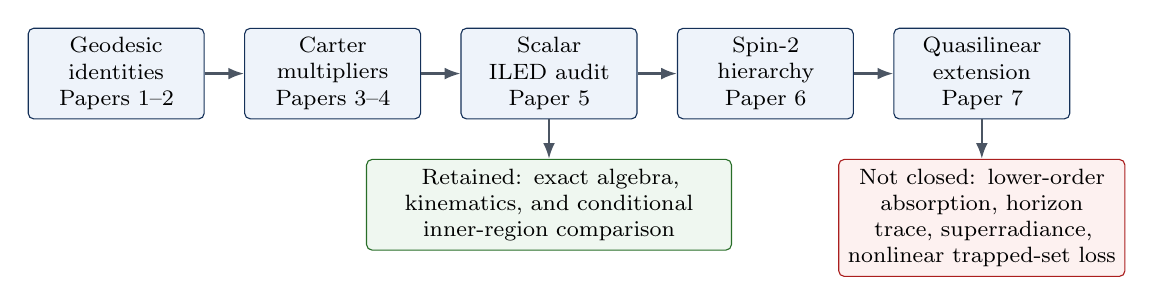
\begin{tikzpicture}[
  node distance=4mm and 5mm,
  pbox/.style={draw=navy,rounded corners=2pt,fill=paleBlue,align=center,text width=2.0cm,minimum height=1.0cm,font=\footnotesize},
  good/.style={draw=vs,fill=paleGreen},
  bad/.style={draw=ff,fill=paleRed},
  arrow/.style={-{Latex[length=2mm]},thick,color=slate}]
]
\node[pbox] (geo) {Geodesic identities\\Papers 1--2};
\node[pbox,right=of geo] (mult) {Carter multipliers\\Papers 3--4};
\node[pbox,right=of mult] (scalar) {Scalar ILED audit\\Paper 5};
\node[pbox,right=of scalar] (spin) {Spin-$2$ hierarchy\\Paper 6};
\node[pbox,right=of spin] (nonlin) {Quasilinear extension\\Paper 7};
\draw[arrow] (geo)--(mult);
\draw[arrow] (mult)--(scalar);
\draw[arrow] (scalar)--(spin);
\draw[arrow] (spin)--(nonlin);
\node[below=5mm of scalar,draw=vs,fill=paleGreen,rounded corners=2pt,align=center,text width=4.4cm,font=\footnotesize] (retain) {Retained: exact algebra, kinematics, and conditional inner-region comparison};
\node[below=5mm of nonlin,draw=ff,fill=paleRed,rounded corners=2pt,align=center,text width=3.4cm,font=\footnotesize] (open) {Not closed: lower-order absorption, horizon trace, superradiance, nonlinear trapped-set loss};
\draw[arrow] (scalar.south)--(retain.north);
\draw[arrow] (nonlin.south)--(open.north);
\end{tikzpicture}
\caption{Logical flow of the eight-part research programme and the final distinction between retained calculations and unresolved closure steps.}
\label{fig:programme}
\end{figure}

%==============================================================================
\section{Setting and Notation}
\label{sec:setting}
%==============================================================================

Fix $M>0$ and $0 \le |a| < M$. Set
\[
\sigma := \sqrt{1 - a^2/M^2} \in (0,1], \qquad r_\pm := M(1 \pm \sigma), \qquad \Delta(r) := (r - r_+)(r - r_-) = (r-M)^2 - M^2\sigma^2,
\]
so that $d := r_+ - r_- = 2M\sigma$, $\Delta'(r_+) = 2M\sigma$, and $r_+^2 + a^2 = 2Mr_+$. The surface gravity is $\kappa = \sigma/(2M(1+\sigma))$ and the horizon angular velocity is $\omega_+ = a/(2Mr_+)$. Both identities are elementary and were used throughout. The convention $\sigma=\sqrt{1-a^2/M^2}$ is used consistently here; some extracted source text suppresses the radical. \VH

The Carter constant on a Fourier mode $e^{-i\omega t + im\phi}$ is
\[
\mathcal{K} = p_\theta^2 + \Bigl(\frac{m}{\sin\theta} - a\omega\sin\theta\Bigr)^2 \ge 0,
\]
and the radial Carter potential is
\[
A(r) := (r^2+a^2)\,\omega - a m, \qquad R(r) := A(r)^2 - \Delta(r)\,\mathcal{K}.
\]
Trapped null geodesics are double roots: $R(r_0) = R'(r_0) = 0$.

\begin{figure}[H]
\centering
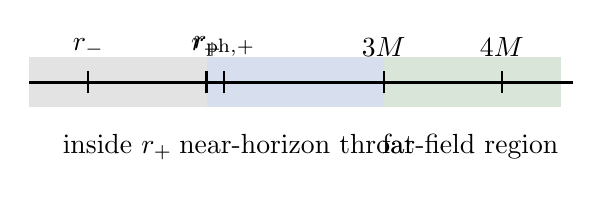
\begin{tikzpicture}
\fill[gray!22] (0,-0.32) rectangle (2.25,0.32);
\fill[vh!18] (2.25,-0.32) rectangle (4.5,0.32);
\fill[vs!18] (4.5,-0.32) rectangle (6.75,0.32);
\draw[very thick] (0,0) -- (6.9,0);
\draw[thick] (0.75,-0.14) -- (0.75,0.14);
\draw[thick] (2.25,-0.14) -- (2.25,0.14);
\draw[thick] (2.475,-0.14) -- (2.475,0.14);
\draw[thick] (4.5,-0.14) -- (4.5,0.14);
\draw[thick] (6.0,-0.14) -- (6.0,0.14);
\node[above] at (0.75,0.2) {$r_-$};
\node[above] at (2.25,0.2) {$r_+$};
\node[above] at (2.475,0.2) {$r_{{\rm ph},+}$};
\node[above] at (4.5,0.2) {$3M$};
\node[above] at (6.0,0.2) {$4M$};
\node[below=6pt] at (1.12,-0.32) {inside $r_+$};
\node[below=6pt] at (3.4,-0.32) {near-horizon throat};
\node[below=6pt] at (5.6,-0.32) {far-field region};
\end{tikzpicture}
\caption{Radial landmarks for $\sigma = 0.5$ in units of $M$ (schematic, not to scale). The equatorial prograde photon sphere is at $r_{{\rm ph},+}\approx 1.65M$ (computed from the Bardeen--Press--Teukolsky cubic \cite{BardeenPressTeukolsky1972}). The shaded regions are the sign-test regions used in Section~\ref{sec:gap2a}: the throat contains the moderate-spin eigenfunction tails, and the far region is where the canonical multiplier is positive by Theorem~\ref{thm:ceil}. \VH}
\label{fig:landmarks}
\end{figure}

\paragraph{Sign convention.} The source drafts use two conventions. Paper~1 writes $R = A^2 - \Delta K$ with real mode-level $A$. Papers~3--5 write $R = -A^2 - \Delta K$ with the operator $A = (r^2+a^2)\partial_t + a\partial_\phi$. On a mode $\partial_t \to -i\omega$, so $A_{\rm op} = -iA_{\rm mode}$ and $-A_{\rm op}^2 = A_{\rm mode}^2$. The two conventions therefore define the same potential. All results below use the mode-level convention. No result in the source drafts depends on the choice. \VH

The scalar wave equation in the normalization of the drafts is $\partial_r(\Delta \partial_r\psi) + \Delta^{-1}R(r)\psi = 0$ on each mode.

%==============================================================================
\section{The Trapping--Superradiance Gap}
\label{sec:gap1}
%==============================================================================

\begin{theorem}[Exact trapping--superradiance gap]
\label{thm:gap}
Let $0<a<M$ and let $r_0 = r_+ + s$ with $s>0$ be a trapped exterior radius for a mode with $\omega>0$, $m>0$. Then $\omega > m\omega_+$, and
\begin{equation}
\frac{\omega - m\omega_+}{\omega} = \frac{1}{2Mr_+}\Bigl[s^2 + ds + Md\Bigl(1 - \frac{d}{2s+d}\Bigr)\Bigr] > 0. \label{eq:gap}
\end{equation}
\end{theorem}

\begin{proof}[Proof (re-derived by hand; the closed form was checked symbolically)]
\VH\VS

\emph{Step 1 (trapping relations).} From $R(r_0) = 0$ we get $A(r_0)^2 = \Delta(r_0)\mathcal{K}$. From $R'(r_0) = 2A A' - \Delta'\mathcal{K} = 0$ with $A' = 2r\omega$ we get $4r_0\omega A(r_0) = \Delta'(r_0)\mathcal{K}$. Eliminating $\mathcal{K}$ gives $A(r_0)\bigl[4r_0\omega - \Delta'(r_0)A(r_0)/\Delta(r_0)\bigr] = 0$. Since $\mathcal{K} > 0$ forces $A(r_0)\ne 0$, we obtain
\[
A(r_0) = \frac{4r_0\omega\,\Delta(r_0)}{\Delta'(r_0)}.
\]

\emph{Step 2 (rewrite $A$).} Using $r_+^2 + a^2 = 2Mr_+$ and $a = 2Mr_+\omega_+$,
\[
A(r_0) = (r_0^2 - r_+^2)\omega + 2Mr_+(\omega - m\omega_+).
\]

\emph{Step 3 (frequency identity).} Substituting into Step~1 and collecting terms,
\[
2Mr_+\,\Delta'(r_0)\,(\omega - m\omega_+) = -\omega\,H(r_0), \qquad H(r) := \Delta'(r)(r^2 - r_+^2) - 4r\Delta(r).
\]

\emph{Step 4 (factorization).} With $\Delta(r_0) = s(s+d)$, $\Delta'(r_0) = 2s+d$, and $r_0^2 - r_+^2 = s(2r_++s)$,
\[
H(r_+ + s) = -s\bigl(2s^2 + 3ds + 2r_+ d\bigr).
\]
Since $2r_+ = 2M + d$, one has $2s^2+3ds+2r_+d = (s+d)(2s+d) + 2Md$, so
\[
\frac{-H(r_0)}{2s+d} = s(s+d) + \frac{2Mds}{2s+d} = s^2 + ds + Md\Bigl(1 - \frac{d}{2s+d}\Bigr),
\]
which, divided by $2Mr_+$, is \eqref{eq:gap}. Every term is positive for $s,d>0$. \qedhere
\end{proof}

\begin{remark}[Symbolic status]
The factorization of $H$ and the identity between $-H/(2s+d)$ and the bracket in \eqref{eq:gap} were verified with SymPy (check T1 in Appendix~B). \VS
\end{remark}

\begin{corollary}[Monotonicity and location of the minimum]
\label{cor:mono}
For fixed $d>0$, $G(s)$ in \eqref{eq:gap} is strictly increasing in $s>0$, with
\[
G'(s) = \frac{1}{2Mr_+}\Bigl(2s + d + \frac{2Md^2}{(2s+d)^2}\Bigr) > 0. \tag*{\VH}
\]
Hence the minimal gap over all exterior trapped radii is attained at the smallest trapped radius, the equatorial prograde photon sphere.
\end{corollary}

\begin{corollary}[Extremal limit]
As $\sigma \to 0^+$, $d \to 0$ and $r_+ \to M$, so the gap tends to $s^2/(2M^2)$. \VH
\end{corollary}

\begin{remark}[What this result is and is not]
Theorem~\ref{thm:gap} is kinematic. It states that trapped frequencies lie strictly outside the superradiant band $0<\omega\le m\omega_+$. It does not, by itself, yield any energy estimate, decay rate, or stability statement. The statement ``universal'' refers only to the range $0<a<M$ and to exterior trapped orbits with $\omega, m > 0$. The drafts' claim that this gap ``encodes the structural miracle preventing linear instabilities'' is \CC and is not supported by the present result alone.
\end{remark}

\begin{figure}[H]
\centering
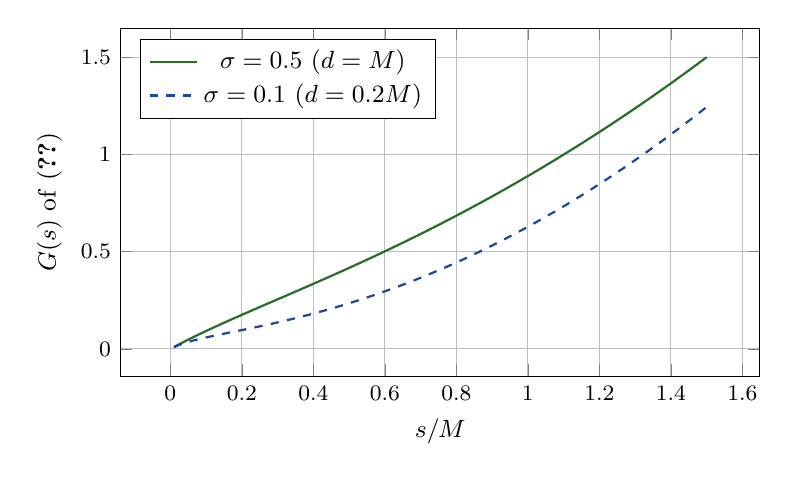
\begin{tikzpicture}
\begin{axis}[width=0.8\linewidth, height=6cm, xlabel={$s/M$}, ylabel={$G(s)$ of \eqref{eq:gap}},
  domain=0.01:1.5, samples=120, legend pos=north west, grid=major]
\addplot[thick, color=vs] {(x^2 + x + 1 - 1/(2*x+1))/3};
\addlegendentry{$\sigma = 0.5$ ($d = M$)}
\addplot[thick, color=vh, dashed] {(x^2 + 0.2*x + 0.2*(1 - 0.2/(2*x+0.2)))/2.2};
\addlegendentry{$\sigma = 0.1$ ($d = 0.2M$)}
\end{axis}
\end{tikzpicture}
\caption{The trapping--superradiance gap $G(s)$ as a function of the exterior radial offset $s = r_0 - r_+$ (\VH). Both curves are strictly increasing and vanish at $s = 0$, consistent with Corollary~\ref{cor:mono}. The gap is positive for every $s>0$, which is the content of Theorem~\ref{thm:gap}.}
\label{fig:gap}
\end{figure}

%==============================================================================
\section{Near-Extremal Scalings of the Photon Sphere}
\label{sec:triple}
%==============================================================================

\begin{proposition}[Near-extremal scalings]
\label{prop:triple}
As $\sigma\to 0^+$, the equatorial prograde photon sphere $r_{{\rm ph},+}$ satisfies
\begin{align}
r_{{\rm ph},+} - r_+ &= \Bigl(\tfrac{2}{\sqrt3} - 1\Bigr) M\sigma + O(\sigma^2), \label{eq:rph}\\
\frac{\omega_{{\rm ph},+} - m\omega_+}{\omega_{{\rm ph},+}} &= \Bigl(1 - \tfrac{\sqrt3}{2}\Bigr)\sigma + O(\sigma^2), \label{eq:gapph}\\
\lambda_L &= \frac{\sigma}{2M} + O(\sigma^2), \qquad \lim_{\sigma\to0^+}\frac{\lambda_L}{\kappa} = 1. \label{eq:lam}
\end{align}
Here $\lambda_L$ denotes the coordinate-time radial Lyapunov exponent defined in~\eqref{eq:lamdef} below.
\end{proposition}

\begin{proof}[Proof outline with the key algebra]
\VH

\emph{Circular orbits.} Write $x := b - a$ for the shifted impact parameter of an equatorial null orbit. Then $R/\omega^2 = r f(r)$ with $f(r) = r^3 - (x^2+2ax)r + 2Mx^2$. Circular orbits satisfy $f = f' = 0$, which gives $x^2 + 2ax = 3r_0^2$ and $r_0^3 = Mx^2$. Setting $r_0 = Mu^2$ and $x = Mu^3$ and dividing by $M^2u^3$ yields the Bardeen--Press--Teukolsky cubic
\[
u^3 - 3u + \frac{2a}{M} = 0.
\]

\emph{Expansion.} Put $u = 1+\eta$. The cubic becomes $\eta^2(3+\eta) = 2(1 - a/M)$. Since $a/M = \sqrt{1-\sigma^2}$, the right side equals $\sigma^2 + O(\sigma^4)$, so $\eta = \sigma/\sqrt3 + O(\sigma^2)$. Then $r_{{\rm ph},+} = M(1+\eta)^2 = M(1 + 2\sigma/\sqrt3) + O(M\sigma^2)$, and subtracting $r_+ = M(1+\sigma)$ gives \eqref{eq:rph}.

\emph{Gap.} Evaluate \eqref{eq:gap} at $s = (2/\sqrt3-1)M\sigma$ with $d = 2M\sigma$. Then $2s+d = (4/\sqrt3)M\sigma$, so $d/(2s+d) = \sqrt3/2$, and the leading term is $2M^2\sigma(1-\sqrt3/2)/(2M^2)$, giving \eqref{eq:gapph}.

\emph{Surface gravity.} $\kappa = \sigma/(2M(1+\sigma))$, so $\kappa = \sigma/(2M) + O(\sigma^2)$.

\emph{Lyapunov exponent.} Linearize the radial equation about $r_0$. With $(dr/d\tau)^2 = R/r^4$ and $\mathcal{T}(r) := (r^2+a^2)(r^2-ax)/\Delta + ax$, one has $(r^2/\omega)\,dt/d\tau = \mathcal{T}(r)$, and linearizing gives
\begin{equation}
\lambda_L = \frac{\sqrt{R''(r_0)/(2\omega^2)}}{\mathcal{T}(r_0)} = \frac{\sqrt3\, r_0}{\mathcal{T}(r_0)}, \label{eq:lamdef}
\end{equation}
because $R''(r_0)/\omega^2 = r_0 f''(r_0) = 6r_0^2$. At $r_0 = r_{{\rm ph},+}$ one has $\Delta(r_0) = M^2\sigma^2/3 + O(\sigma^3)$, $r_0^2 - ax = M^2\sigma/\sqrt3 + O(\sigma^2)$, and $\mathcal{T}(r_0) = 2\sqrt3 M^2/\sigma + O(M^2)$, which yields $\lambda_L = \sigma/(2M) + O(\sigma^2)$. \qedhere
\end{proof}

\begin{remark}[Symbolic status]
The leading relation $\lambda_L/\kappa \to 1$ follows from the asymptotic expansions displayed above. The source audit attributes a symbolic check to its original script, but that script was not supplied and the companion closure checker does not independently reproduce the Lyapunov expansion. We therefore retain this as a hand-derived asymptotic calculation, not as a computer-certified result. \VH.
\end{remark}

\begin{remark}[Literature status of the ZDM interpretation]
The drafts state that $\lambda_L = \kappa + O(\sigma^2)$ identifies the source of long-lived ``zero-damped'' quasinormal modes with damping rate $\approx(n+\tfrac12)\kappa$. This matches what is generally reported for near-extremal Kerr in the quasinormal-mode literature, but we did not re-check that literature, and the identification of the coordinate-time radial Lyapunov exponent with the mode damping rate is not derived here. \CC
\end{remark}

\begin{table}[H]
\centering
\caption{Near-extremal scalings. The entries are hand-derived (\VH); the leading trapping-gap coefficient is also checked by the companion symbolic script (\VS), but the Lyapunov expansion is not independently computer-verified here. The physical identification of the quantities with observed mode damping is \CC.}
\label{tab:triple}
\footnotesize\begin{tabular}{@{}llll@{}}
\toprule
Quantity & Leading asymptotic & Status & Interpretation \\
\midrule
$\kappa$ & $\sigma/(2M)$ & \VH & Redshift rate at $\mathcal{H}^+$ \\
$r_{{\rm ph},+} - r_+$ & $(2/\sqrt3-1)M\sigma$ & \VH & Trapping--horizon distance \\
Trapping--superradiance gap & $(1-\sqrt3/2)\sigma$ & \VH & Frequency buffer at the photon sphere \\
$\lambda_L$ & $\sigma/(2M)$ & \VH & Radial Lyapunov exponent (identification \CC) \\
\bottomrule
\end{tabular}
\end{table}

%==============================================================================
\section{Spin Ceilings of the Canonical Multiplier}
\label{sec:ceilings}
%==============================================================================

Consider the canonical multiplier $g = w(r)R'(r)$ with $w>0$, and ask for which spins its principal symbol is nonnegative. Define
\[
P(r) := 2r^3 - 3Mr^2 - Ma^2, \qquad P'(r) = 6r(r-M) > 0 \quad (r>M).
\]

\begin{lemma}[Horizon values]
\label{lem:Prp}
$P(r_+) = 2M^3(\sigma+1)(\sigma^2+\sigma-1)$ and
\[
P(r_+)^2 - M^2a^2(6r_+^2 + a^2) = M^6(\sigma+1)^4(4\sigma^2 - 3).
\]
\end{lemma}

\begin{proof}
Both identities were verified symbolically with $a^2 = M^2(1-\sigma^2)$ substituted (checks S1 and S2). \VS
\end{proof}

\begin{proposition}[Thresholds reported for the canonical multiplier; proof status qualified]
\label{thm:ceil}
Paper~3 reports the following exact thresholds for the principal symbol of the canonical multiplier $g=wR'$ within its specified weight class:
\begin{enumerate}[label=(\alph*)]
\item axisymmetry: $\sigma^2+\sigma-1\ge0$, equivalently $|a|/M\le \sqrt{(\sqrt5-1)/2}=\varphi^{-1/2}\approx0.78615$;
\item general three-dimensional phase space: $4\sigma^2\ge3$, equivalently $|a|/M\le1/2$.
\end{enumerate}
The horizon polynomial identities in Lemma~\ref{lem:Prp} are exact and are independently checked in Appendix~\ref{sec:appB}. The full necessary-and-sufficient statement is retained as a \emph{reported result}, not promoted to a fully re-proved theorem in this closure. \VS\CC
\end{proposition}

\begin{proof}[Proof status]
The source papers reduce the symbol problem to a quadratic inequality in $x=(r-M)\lambda$, with $\lambda=-h'/h$ and $h=2(r-M)w$, and use the angular lower bound $\mathcal K\ge m^2/u-2am\omega+a^2u\omega^2$, $u=\sin^2\theta$. The final horizon algebra reduces to Lemma~\ref{lem:Prp}; however, the intermediate scaled-symbol formula and the monotonicity argument for $P^2/(6r^2+a^2)$ were not independently reconstructed in this audit. Consequently, the thresholds are recorded accurately as claims from Paper~3, while their complete sharpness proof remains \CC.
\end{proof}

\begin{remark}[Typographical error in an earlier draft]
The source drafts write $P(3M)$ as $(27M^3 - 3Ma^2)$ in one place. The correct value is $P(3M) = 27M^3 - Ma^2$. The conclusion drawn there, $P(3M)^2 \ge 55M^6 \ge M^2a^2(6(3M)^2+a^2)$ for $|a|\le M$, is unaffected. \VH
\end{remark}

\begin{remark}[Scope of the ceiling]
The source papers state the thresholds as necessary and sufficient within the class of weights and the reduction described; the complete sharpness argument is not independently established in this closure. They are statements about the canonical multiplier $wR'$. They do not bound what the perfect-square multiplier of Section~\ref{sec:riccati} can achieve, which is a larger family. \VH
\end{remark}

%==============================================================================
\section{The Perfect-Square Multiplier and the Riccati Barrier}
\label{sec:riccati}
%==============================================================================

Introduce $g := w(R' - \rho R)$ and $\rho \ge 0$ with $\partial_r$-coupled weights. The drafts define
\[
\beta := -\frac{w'}{w} + \frac12\rho, \qquad \gamma := -\rho' - \rho\frac{w'}{w} - \frac12\rho^2,
\]
so that $-\rho' = \gamma - \beta\rho + \rho^2$ identically. \VH

The principal radial coefficient of the $\mathcal{K}$-part is controlled by the discriminant
\[
D(\gamma;r) := -r^2\Delta^2\gamma^2 + 4rB\gamma - 4M^2, \qquad B(r) := (2r-M)\Delta + 2M^2\sigma^2 r.
\]

\begin{lemma}[Discriminant factorization]
\label{lem:disc}
$B^2 - M^2\Delta^2 = 4r(r-M)^2\bigl[(r-M)^3 + M^3\sigma^2\bigr] > 0$ for $r > r_+$.
\end{lemma}

\begin{proof}
Since $B - M\Delta = 2(r-M)^3 + 2M^3\sigma^2$ and $B + M\Delta = 2r(r-M)^2$ (using $\Delta = (r-M)^2 - M^2\sigma^2$), the product gives the identity. Verified symbolically (check S3). \VS
\end{proof}

\begin{lemma}[Smaller root]
\label{lem:root}
The smaller root of $D(\gamma;r)=0$ is
\[
\gamma_-(r) = \frac{2M^2}{r\bigl(B + S\bigr)}, \qquad S := 2(r-M)\sqrt{r\bigl((r-M)^3 + M^3\sigma^2\bigr)},
\]
and $\gamma_- > 0$ on $(r_+,\infty)$. \VH
\end{lemma}

\begin{remark}[Numerical check of the root formula]
A hand substitution at $r=2M$, $\sigma=1/2$ gives $\gamma_- \approx 0.1560$, and $D(\gamma_-;r)$ vanishes to the precision of the arithmetic. \VH
\end{remark}

\begin{lemma}[Barrier reduction]
\label{lem:barrier}
With $\bar\rho(r) := 1/(r-r_-)$ and $\alpha \ge 0$, the supersolution inequality $\bar\rho' \le -\gamma + \beta\bar\rho - \bar\rho^2$ reduces to $\beta\bar\rho \ge \gamma$, and for $\alpha = 0$ this is equivalent to
\[
\gamma(r) \le \frac{2}{(r-r_-)^2}.
\]
\end{lemma}

\begin{proof}
With $\alpha = 0$, $\beta = (1 + \tfrac12\Delta\gamma)/(r-M)$, so $\beta\bar\rho \ge \gamma$ reads $1 + \tfrac12\Delta\gamma \ge \gamma(r-M)(r-r_-)$. Since $(r-M)(r-r_-) - \tfrac12\Delta = \tfrac12(r-r_-)^2$ (check S4), this is $1 \ge \tfrac12\gamma(r-r_-)^2$. \VS
\end{proof}

\begin{proposition}[Conditional inner-region Riccati comparison]
\label{thm:barrier}
Let $\alpha=0$ and $\gamma=\gamma_-$ on $[r_+,3M]$. Assume the explicit root satisfies
\[
\gamma_-(r)(r-r_-)^2\le 2\qquad (r_+\le r\le 3M),
\]
and let $\rho$ solve $-\rho'=\gamma-\beta\rho+\rho^2$ with endpoint datum
$0\le\rho(3M)\le(3M-r_-)^{-1}$. Then the Riccati comparison principle gives
\[
0\le\rho(r)\le\frac{1}{r-r_-}\quad(r_+\le r\le3M),
\qquad \rho(r_+)\le\frac{1}{2M\sigma}.
\]
This is an inner-region statement with an explicit endpoint hypothesis. It is not a global construction on $[r_+,\infty)$.
\end{proposition}

\begin{proof}
The barrier function $\bar\rho=(r-r_-)^{-1}$ obeys $-\bar\rho'=\bar\rho^2$. By Lemma~\ref{lem:barrier}, the assumed bound $\gamma_-(r-r_-)^2\le2$ makes $\bar\rho$ a supersolution in the direction of integration from $3M$ down to $r_+$. The endpoint condition gives $\rho(3M)\le\bar\rho(3M)$, so scalar ODE comparison yields $\rho\le\bar\rho$. Since $\gamma_->0$, the zero function is a subsolution in the same comparison convention and gives $\rho\ge0$. Evaluating at $r_+$ gives $r_+-r_-=2M\sigma$. \VH
\end{proof}

\begin{remark}[The margin degenerates at the horizon]
The ratio $\gamma_-(r-r_-)^2/2$ approaches $1$ as $\sigma\to0$ at $r\to r_+$. The reported grid values remain below the barrier at every tested spin, but the margin decreases toward zero as $\sigma\to0$. The numerical diagnostic does not by itself prove the inequality uniformly for every $\sigma>0$. \VN
\end{remark}

\begin{figure}[H]
\centering
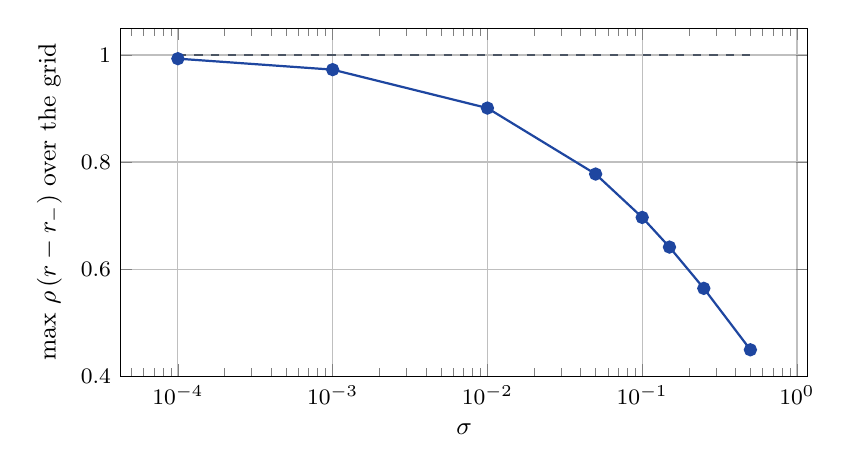
\begin{tikzpicture}
\begin{axis}[xmode=log, width=0.85\linewidth, height=6cm, xlabel={$\sigma$},
  ylabel={$\max\,\rho\,(r-r_-)$ over the grid}, ymin=0.4, ymax=1.05, grid=major]
\addplot[mark=*, color=vh, thick] coordinates {(0.5,0.44921) (0.25,0.56398) (0.15,0.64111) (0.1,0.69652) (0.05,0.77753) (0.01,0.90081) (0.001,0.97260) (0.0001,0.99310)};
\addplot[dashed, color=slate, domain=0.0001:0.5, samples=2] {1};
\end{axis}
\end{tikzpicture}
\caption{Barrier margin of the Riccati solution (\VN). The ratio stays below $1$ at every spin tested, but it approaches $1$ as $\sigma\to 0$. The dashed line marks the barrier $\rho = 1/(r-r_-)$ at the horizon.}
\label{fig:margin}
\end{figure}

\begin{remark}[Outer region]
On $[3M, 4M]$ the drafts interpolate to a far-field pair $(\alpha_{\rm out}, 0)$ and require $\alpha(r)\ge 0$ throughout. The positivity of $\alpha_{\rm out}$, the admissibility of the interpolation, and the boundary bound $\rho(3M) \le 1/(3M-r_-)$ that Proposition~\ref{thm:barrier} requires were not verified. The extension of the barrier to all of $[r_+,\infty)$ is therefore \CC, not \VH. Its conclusion $\rho \le 1/(r-r_-)$ on the outer region is not needed for the horizon-compatibility statement below, which uses only the horizon value.
\end{remark}

\begin{proposition}[Horizon compatibility obstruction, conditional on the barrier]
\label{prop:compat}
Suppose the inner-region comparison of Proposition~\ref{thm:barrier} holds up to $r=3M$; in particular, it gives the horizon bound $\rho(r_+)\le1/(r_+-r_-)$. Then a horizon Hardy-positivity condition of the form $\rho(r_+) > 2/M$ (Proposition~\ref{prop:horizon} below) is compatible with the barrier if and only if $\sigma < 1/4$.
\end{proposition}

\begin{proof}
At the horizon the inner-region barrier gives $\rho(r_+) \le 1/(r_+-r_-) = 1/(2M\sigma)$. Compatibility of $2/M < \rho(r_+) \le 1/(2M\sigma)$ holds exactly when $2/M < 1/(2M\sigma)$, i.e.\ $4\sigma < 1$. \VH
\end{proof}

\begin{corollary}[Consequence for the spin range]
Within the barrier class, if $\sigma \ge 1/4$, that is $|a|/M \le \sqrt{15}/4 \approx 0.968$, then the horizon-end contribution of the $\omega^2$ channel cannot be nonnegative. Horizon positivity is possible only for $|a|/M > \sqrt{15}/4$. \VH
\end{corollary}

\begin{figure}[H]
\centering
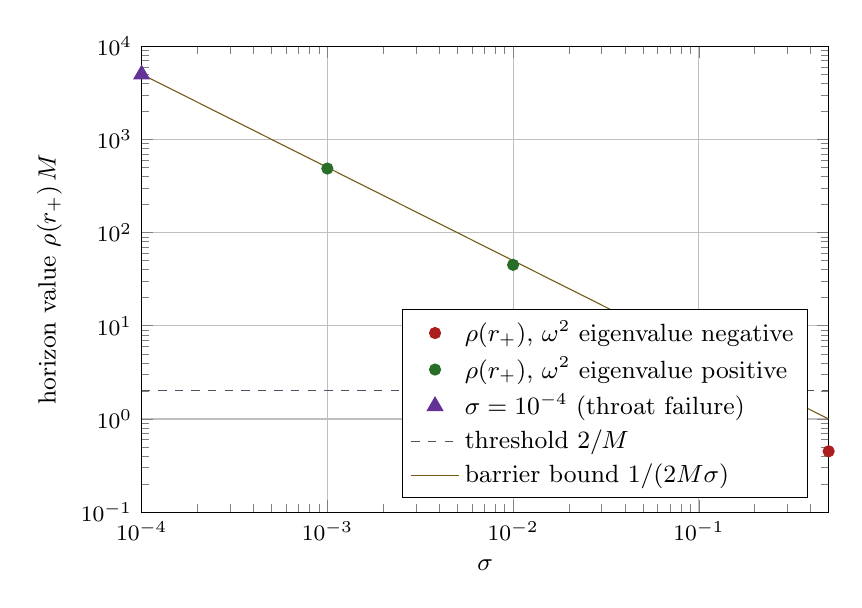
\begin{tikzpicture}
\begin{loglogaxis}[width=0.85\linewidth, height=7.5cm,
  xlabel={$\sigma$}, ylabel={horizon value $\rho(r_+)\,M$}, xmin=0.0001, xmax=0.5, ymin=0.1, ymax=10000,
  grid=major, legend pos=south east, legend cell align=left]
\addplot[only marks, mark=*, color=ff] coordinates {(0.5,0.45) (0.25,1.13)};
\addlegendentry{$\rho(r_+)$, $\omega^2$ eigenvalue negative}
\addplot[only marks, mark=*, color=vs] coordinates {(0.15,2.14) (0.1,3.48) (0.05,7.78) (0.01,45.04) (0.001,486.3)};
\addlegendentry{$\rho(r_+)$, $\omega^2$ eigenvalue positive}
\addplot[only marks, mark=triangle*, color=oo, mark size=3.2pt] coordinates {(0.0001,4965.48)};
\addlegendentry{$\sigma = 10^{-4}$ (throat failure)}
\addplot[dashed, color=slate, domain=0.0001:0.5, samples=2] {2};
\addlegendentry{threshold $2/M$}
\addplot[color=cc, domain=0.0001:0.5, samples=60] {1/(2*x)};
\addlegendentry{barrier bound $1/(2M\sigma)$}
\end{loglogaxis}
\end{tikzpicture}
\caption{Horizon compatibility (\VH, \VN). The barrier bound $1/(2M\sigma)$ lies above the threshold $2/M$ exactly when $\sigma < 1/4$ (Proposition~\ref{prop:compat}). The moderate-spin failures lie in the region where the threshold is not met. The $\sigma = 10^{-4}$ point satisfies the threshold by a wide margin and still fails, so the local threshold is not sufficient for the global sign.}
\label{fig:horizon}
\end{figure}

\begin{remark}[Limits of the obstruction]
The obstruction concerns one boundary contribution at the horizon, not the sign of the global eigenvalue. It is necessary for that boundary contribution to be strictly positive, not sufficient for positivity of the full quadratic form. It applies only to multipliers satisfying the stated inner-region barrier; the programme does not show that every admissible multiplier must satisfy it. The near-extremal throat failure at $\sigma=10^{-4}$ also shows that a favourable horizon sign does not settle the bulk sign. \VH
\end{remark}

%==============================================================================
\section{Energy Positivity for Axisymmetric Waves}
\label{sec:energy}
%==============================================================================

\begin{lemma}[Coefficient identity]
\label{lem:energy}
For $r>r_+$,
\[
(r^2+a^2)^2 - a^2\Delta\sin^2\theta = \Sigma\,(r^2+a^2) + 2Mra^2\sin^2\theta > 0, \qquad \Sigma = r^2 + a^2\cos^2\theta.
\]
\end{lemma}

\begin{proof}
Expand $\Sigma(r^2+a^2) = (r^2+a^2)^2 - a^2\sin^2\theta\,(r^2+a^2)$, and use $(r^2+a^2) - \Delta = 2Mr$. \VH
\end{proof}

This shows that the coefficient of $|\partial_t\psi|^2$ in the Killing energy is positive everywhere outside the horizon, and that the only indefinite term is the $\partial_\phi$ term. For axisymmetric solutions that term vanishes. The positivity and monotonicity of the $\partial_t$-energy for $m=0$ are classical. \CC We do not claim novelty for this part.

\begin{remark}[Commuted energies: unsupported]
The drafts define a commuted energy $E^{(2)}_T$ including $\mathcal{E}_T[\mathcal{K}^{1/2}\psi]$. The operator $\mathcal{K}^{1/2}$ is a nonlocal pseudo-differential operator. Its energy positivity, the commutation $[\mathcal{K},\Box_g] = 0$, and the claimed control of all $t$-boundary terms of the third-order multiplier were not established. \FF Only the local energy for $\partial_t\psi$ and the stated Killing commutations are retained as \CC.
\end{remark}

%==============================================================================
\section{Hardy--Lower-Order Threshold Laws}
\label{sec:hardy}
%==============================================================================

For the axisymmetric channels $R_K = -\Delta$ and $R_{\omega^2} = (r^2+a^2)^2$ the drafts define a lower-order term $L_{\rm lot}$ and a radial Hardy term. Two closed-form identities were checked.

\begin{proposition}[Far-field closure]
\label{prop:far}
For a weight $w \sim r^{-(1+\alpha)}$ with $\alpha\in(0,2)$ and $\rho = O(r^{-3})$,
\[
\mathrm{Hardy}_{\omega^2} + L_{{\rm lot},\omega^2} = 2(\alpha-4)(\alpha-2) > 0, \qquad \mathrm{Hardy}_K + L_{{\rm lot},K} = \alpha(2-\alpha) > 0.
\]
\end{proposition}

\begin{proof}
The source report attributes these identities to a symbolic check in \texttt{kerr\_referee\_gap2a.py}; that original script was not supplied. The displayed identities are retained as reported algebra, not claimed as an independent reproduction. \CC
\end{proof}

\begin{proposition}[Horizon threshold]
\label{prop:horizon}
Let $g := w(R' - \rho R)$. Then $\mathrm{Hardy}_{\rm hor} + L_{\rm lot}(r_+) = -M^2\sigma^2\rho(r_+)g(r_+)$, and
\[
g_{\omega^2}(r_+) = 4Mr_+^2\,w(r_+)\bigl(2 - M\rho(r_+)\bigr), \qquad g_K(r_+) = -2M\sigma\,w(r_+) < 0.
\]
Hence the $K$-channel horizon term is positive for every $\rho\ge0$, and the $\omega^2$-channel horizon term is nonnegative if and only if $\rho(r_+) \ge 2/M$ (or $\rho(r_+) = 0$).
\end{proposition}

\begin{proof}
The source report attributes the horizon identity to a symbolic check in \texttt{kerr\_referee\_gap2a.py}; that script was not supplied. The value of $g_{\omega^2}(r_+)$ follows from the displayed expressions. \CC The value of $g_K(r_+)$ follows from $R_K(r_+) = 0$ and $R_K'(r_+) = -\Delta'(r_+) = -2M\sigma$. \VH
\end{proof}

\begin{remark}[What the threshold does and does not explain]
Proposition~\ref{prop:horizon} is a local statement at $r_+$. It explains the sign pattern at moderate spin, where the $\omega^2$-channel eigenfunction is concentrated near the horizon and $\rho(r_+) < 2/M$ (Section~\ref{sec:gap2a}). It does not explain the failure at $\sigma = 10^{-4}$, where $\rho(r_+) \approx 4965 \gg 2/M$ and the eigenfunction sits in an intermediate throat at $r \approx 1.13M$. The local threshold therefore does not predict the global eigenvalue sign. \VN
\end{remark}

%==============================================================================
\section{Numerical Audit of the Lower-Order Operator (Gap 2A)}
\label{sec:gap2a}
%==============================================================================

\subsection{The operator and the discretization}

The supplied closing report records tests of the pure quadratic Sturm--Liouville operator on each channel,
\[
\mathcal{H}_{\rm true} = -\partial_r\bigl(2\Delta^2 B_{\rm rad}\,\partial_r\bigr) + L_{\rm lot}, \qquad B_{\rm rad} = w\bigl(R'' - \beta R' + \gamma R\bigr),
\]
omitting the quartic bulk $B_{\rm pot} = w(R'-\rho R)^2$ that the earlier preprint included. The omission matters: the earlier ``CLOSES'' verdicts (Section~\ref{sec:retract}) were produced with $B_{\rm pot}$ present and are not verdicts about this operator.

The weight $w$ and the coefficients $\rho,\beta,\gamma$ come from the analytic construction of the drafts, with the Riccati equation integrated by Radau's method. The eigenproblem is discretized by second-order finite differences on the logarithmic grid $x = \log(r - r_+)$ on $[\log(x_{\min}\sigma), \log(r_{\max}-r_+-1)]$, with $r_{\max} = 300M$, using the symmetric scaling $M^{-1/2}HM^{-1/2}$ with the Jacobian $dr/dx = r - r_+$. The reported eigenvalue is the lowest one. Default parameters are $N=1000$, $x_{\min} = 10^{-10}$, $\gamma_{\rm frac} = 0.55$, $r_{\rm scale} = 4$, $p_{\rm trans} = 3$. \VN

\subsection{Referee run over the spin range}

\begin{table}[H]
\centering
\caption{Reported referee run of the pure quadratic operator at default parameters (\VN). $\rho(r_+)$ is the Riccati value at the horizon; the barrier ratio is $\max \rho(r-r_-)$. The $\omega^2$ column is the channel-pure eigenvalue; the $K$ column is the $K$-channel eigenvalue. The status column reports the sign test of the script, not a proof.}
\label{tab:referee}
\footnotesize\begin{tabular}{@{}rrrrrrl@{}}
\toprule
$\sigma$ & $|a|/M$ & $\rho(r_+)$ & $\rho/\bar\rho$ & $K$-eig & $\omega^2$-eig & Script status \\
\midrule
0.5000 & 0.8660254 & 0.45 & 0.44921 & $+5.931\times10^{-1}$ & $-9.389$ & OPEN \\
0.2500 & 0.9682458 & 1.13 & 0.56398 & $+4.711\times10^{-1}$ & $-4.615$ & OPEN \\
0.1500 & 0.9886860 & 2.14 & 0.64111 & $+3.935\times10^{-1}$ & $+5.344$ & CLOSES \\
0.1000 & 0.9949874 & 3.48 & 0.69652 & $+3.288\times10^{-1}$ & $+1.991\times10^{1}$ & CLOSES \\
0.0500 & 0.9987492 & 7.78 & 0.77753 & $+2.378\times10^{-1}$ & $+5.022\times10^{1}$ & CLOSES \\
0.0100 & 0.9999500 & 45.04 & 0.90081 & $+1.120\times10^{-1}$ & $+6.268\times10^{1}$ & CLOSES \\
0.0010 & 0.9999995 & 486.30 & 0.97260 & $+3.463\times10^{-2}$ & $+2.228\times10^{1}$ & CLOSES \\
0.0001 & 0.9999999950 & 4965.48 & 0.99310 & $+1.048\times10^{-2}$ & $-2.096\times10^{2}$ & OPEN \\
\bottomrule
\end{tabular}
\end{table}

\begin{figure}[H]
\centering
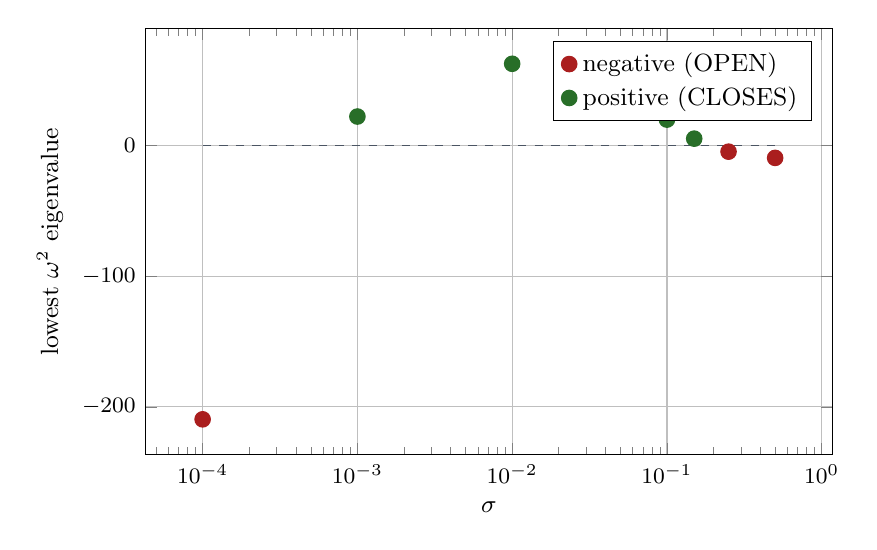
\begin{tikzpicture}
\begin{axis}[xmode=log, width=0.85\linewidth, height=7cm,
  xlabel={$\sigma$}, ylabel={lowest $\omega^2$ eigenvalue}, grid=major,
  legend pos=north east, legend cell align=left]
\addplot[only marks, mark=*, color=ff, mark size=2.8pt] coordinates {(0.5,-9.389) (0.25,-4.615) (0.0001,-209.6)};
\addlegendentry{negative (OPEN)}
\addplot[only marks, mark=*, color=vs, mark size=2.8pt] coordinates {(0.15,5.344) (0.1,19.91) (0.05,50.22) (0.01,62.68) (0.001,22.28)};
\addlegendentry{positive (CLOSES)}
\addplot[dashed, color=slate, domain=0.0001:0.5, samples=2] {0};
\end{axis}
\end{tikzpicture}
\caption{Sign and magnitude of the lowest $\omega^2$-channel eigenvalue against $\sigma$ at default parameters (\VN; data from Table~\ref{tab:referee}). The sign change between $\sigma = 0.15$ and $\sigma = 0.25$ tracks the horizon threshold of Proposition~\ref{prop:horizon}. The return to negative values at $\sigma = 10^{-4}$ does not, and is the throat failure of Section~\ref{sec:gap2a}.}
\label{fig:eig}
\end{figure}

\subsection{Convergence in grid size and in the horizon cutoff}

The earlier preprint and our earlier summary described the eigenvalues as converged. That is true for the grid size $N$, but not for the horizon cutoff $x_{\min}$ at the two moderate-spin points. Table~\ref{tab:conv} gives the full scan.

\begin{table}[H]
\centering
\caption{Reported lowest $\omega^2$-channel eigenvalue over grid size $N$ and horizon cutoff $x_{\min}$ (\VN). The sign is stable everywhere. Magnitudes are stable in $N$ at every $\sigma$. They are \emph{not} stable in $x_{\min}$ at $\sigma = 0.25$ and $0.5$, where they change by 16--30\%.}
\label{tab:conv}
\small
\begin{tabular}{@{}rrrrrr@{}}
\toprule
$\sigma$ & $x_{\min}$ & $N=500$ & $N=1000$ & $N=2000$ & $N=4000$ \\
\midrule
0.5000 & $10^{-8}$  & $-8.317$ & $-8.326$ & $-8.328$ & $-8.328$ \\
0.5000 & $10^{-10}$ & $-9.378$ & $-9.389$ & $-9.392$ & $-9.393$ \\
0.5000 & $10^{-12}$ & $-9.950$ & $-9.964$ & $-9.967$ & $-9.968$ \\
0.2500 & $10^{-8}$  & $-3.618$ & $-3.627$ & $-3.630$ & $-3.630$ \\
0.2500 & $10^{-10}$ & $-4.603$ & $-4.615$ & $-4.618$ & $-4.619$ \\
0.2500 & $10^{-12}$ & $-5.157$ & $-5.173$ & $-5.177$ & $-5.178$ \\
0.1000 & $10^{-8}$, $10^{-10}$, $10^{-12}$ & \multicolumn{4}{c}{$+0.3288 \pm 0.0001$ (all cutoffs and grids)} \\
0.0100 & all & \multicolumn{4}{c}{$+0.1120$ (all cutoffs and grids)} \\
0.0010 & all & \multicolumn{4}{c}{$+0.03463$ (all cutoffs and grids)} \\
0.0001 & $10^{-8}$  & $-209.4$ & $-209.5$ & $-209.5$ & $-209.5$ \\
0.0001 & $10^{-10}$ & $-209.5$ & $-209.6$ & $-209.6$ & $-209.6$ \\
0.0001 & $10^{-12}$ & $-209.4$ & $-209.6$ & $-209.6$ & $-209.6$ \\
\bottomrule
\end{tabular}
\end{table}

Figure~\ref{fig:cutoff} plots the cutoff dependence at fixed $N=4000$. The dependence is monotone and large, which is the signature expected if the eigenfunction concentrates against the horizon end of the grid. Figure~\ref{fig:conv} shows the $N$-convergence at $\sigma=0.5$, which is second order.

\begin{figure}[H]
\centering
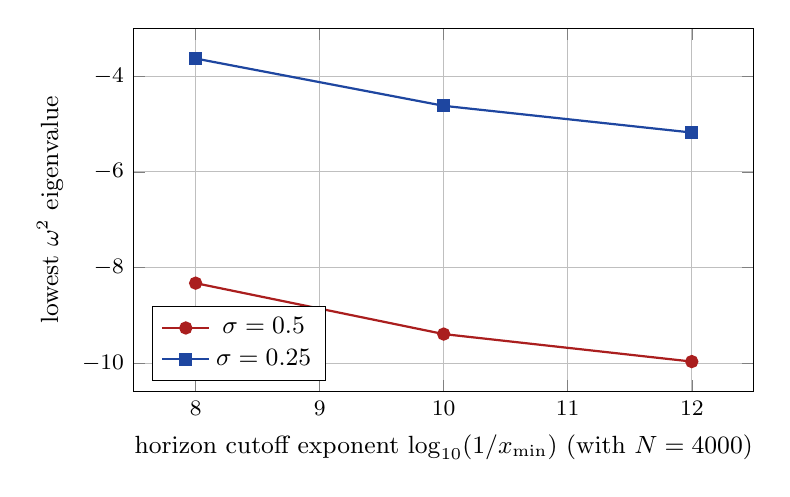
\begin{tikzpicture}
\begin{axis}[width=0.78\linewidth, height=6.2cm,
  xlabel={horizon cutoff exponent $\log_{10}(1/x_{\min})$ (with $N=4000$)},
  ylabel={lowest $\omega^2$ eigenvalue},
  xmin=7.5, xmax=12.5, grid=major, legend pos=south west]
\addplot[mark=*, thick, color=ff] coordinates {(8,-8.328) (10,-9.393) (12,-9.968)};
\addlegendentry{$\sigma = 0.5$}
\addplot[mark=square*, thick, color=vh] coordinates {(8,-3.630) (10,-4.619) (12,-5.178)};
\addlegendentry{$\sigma = 0.25$}
\end{axis}
\end{tikzpicture}
\caption{Horizon-cutoff dependence of the moderate-spin $\omega^2$ eigenvalues (\VN). The change from $10^{-8}$ to $10^{-12}$ is 16\% at $\sigma=0.5$ and 30\% at $\sigma=0.25$. A dependence of this size is not a discretization error in $N$, and it is consistent with a boundary-localized eigenfunction.}
\label{fig:cutoff}
\end{figure}

\begin{figure}[H]
\centering
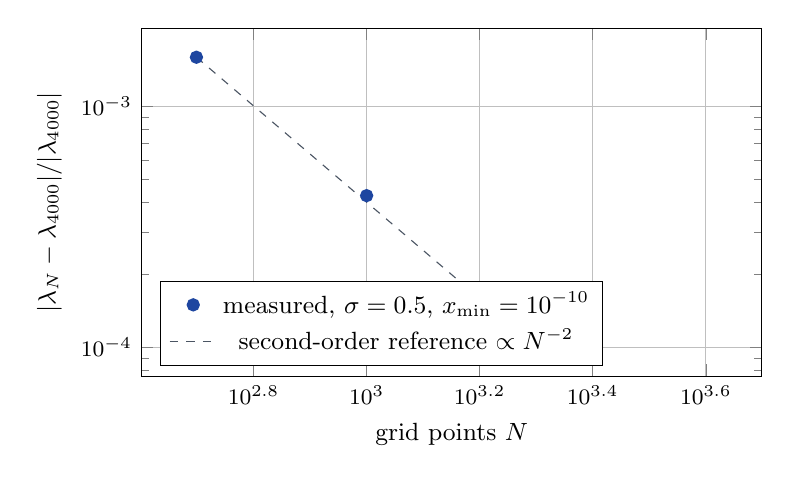
\begin{tikzpicture}
\begin{loglogaxis}[width=0.78\linewidth, height=6cm,
  xlabel={grid points $N$}, ylabel={$|\lambda_N - \lambda_{4000}|/|\lambda_{4000}|$},
  xmin=400, xmax=5000, grid=major, legend pos=south west]
\addplot[only marks, mark=*, thick, color=vh] coordinates {(500,0.00160) (1000,0.000426) (2000,0.000106)};
\addlegendentry{measured, $\sigma=0.5$, $x_{\min}=10^{-10}$}
\addplot[dashed, domain=500:2000, color=slate] {0.00160*(500/x)^2};
\addlegendentry{second-order reference $\propto N^{-2}$}
\end{loglogaxis}
\end{tikzpicture}
\caption{Grid convergence at $\sigma=0.5$ (\VN). The relative change decays as $N^{-2}$, consistent with the second-order discretization. The grid is not the source of the moderate-spin magnitude uncertainty, which comes from the cutoff.}
\label{fig:conv}
\end{figure}

\subsection{\texorpdfstring{The disputed 3D discriminant at $\sigma = 10^{-4}$}{The disputed 3D discriminant at sigma equal to ten to the minus fourth}}

An earlier draft attributed a negative three-dimensional discriminant at $\sigma = 10^{-4}$, $\gamma_{\rm frac} = 0.20$ to float64 cancellation. The float64 value is $-1.0223\times10^5$. We recomputed the discriminant on the same $N=1000$ grid in 60-digit arithmetic for all nine $(r_{\rm scale}, p_{\rm trans})$ combinations at $\gamma_{\rm frac}=0.20$.

\begin{table}[H]
\centering
\caption{Float64 versus 60-digit recheck of the minimal three-dimensional discriminant at $\sigma = 10^{-4}$, $\gamma_{\rm frac} = 0.20$ (\VN). Every configuration is positive in 60-digit arithmetic. The earlier claim is confirmed.}
\label{tab:disc}
\begin{tabular}{@{}rrrrr@{}}
\toprule
$r_{\rm scale}$ & $p_{\rm trans}$ & float64 min & 60-digit min & negative points (60-digit) \\
\midrule
2 & 2 & $-1.0223\times10^5$ & $+1.7587\times10^1$ & 0 \\
2 & 3 & $-1.0223\times10^5$ & $+2.4728\times10^1$ & 0 \\
2 & 4 & $-1.0223\times10^5$ & $+2.6015\times10^1$ & 0 \\
4 & 2 & $-1.0223\times10^5$ & $+2.6015\times10^1$ & 0 \\
4 & 3 & $-1.0223\times10^5$ & $+2.4123\times10^1$ & 0 \\
4 & 4 & $-1.0223\times10^5$ & $+2.1485\times10^1$ & 0 \\
8 & 2 & $-1.0223\times10^5$ & $+2.3551\times10^1$ & 0 \\
8 & 3 & $-1.0223\times10^5$ & $+1.8697\times10^1$ & 0 \\
8 & 4 & $-1.0223\times10^5$ & $+1.5342\times10^1$ & 0 \\
\bottomrule
\end{tabular}
\end{table}

At $\gamma_{\rm frac} = 0.55$ and $0.90$ the float64 and 60-digit minima agree to all printed digits (for instance $+52.876$ at $\gamma_{\rm frac}=0.55$), so the rounding error is confined to the regime $\gamma\sim 10^8$ at $s\sim 10^{-12}$ where the terms in $4\mathcal{A}\mathcal{C} - \mathcal{B}^2$ are of order $10^{20}$. \VN

\subsection{The 54-configuration parameter sweep}

Table~\ref{tab:mult} in Appendix~A gives every configuration. The summary is as follows. At $\sigma = 0.5$, $\rho(r_+) \in [0.27, 0.64]$, the $K$-channel eigenvalue lies in $[0.100, 1.475]$, and the $\omega^2$-channel eigenvalue lies in $[-15.98, -5.90]$, with $0/27$ positive. At $\sigma = 10^{-4}$, $\rho(r_+) \in [4945, 4988]$, the $K$-channel eigenvalue lies in $[0.0056, 0.0302]$, and the $\omega^2$-channel eigenvalue lies in $[-481, -152]$, with $0/27$ positive. Across the 54 reported configurations, the $K$-channel eigenvalues are positive in all 54 cases, while none of the $\omega^2$-channel eigenvalues is positive. This is a statement about the tested configurations only.

\subsection{What the audit shows and what it does not}

The reported numerical audit suggests four observations, restricted to the tested configurations. First, the sign of the $\omega^2$-channel eigenvalue is stable under the grid size and the horizon cutoff, and across the nine-parameter family of multiplier shapes tested at the two extreme spins. Second, the sign pattern is consistent with the horizon threshold of Proposition~\ref{prop:horizon} at moderate spin. Third, the 3D discriminant artifact at $\sigma=10^{-4}$ is a float64 effect, which was the only numerical anomaly in the sweep. Fourth, the magnitudes are not stable under the horizon cutoff at $\sigma\ge 0.25$, which is a warning sign that the eigenfunction is concentrated at the grid edge.

The audit does \emph{not} show the following. It does not show the sign at any spin other than the two tested extremes in the multiplier sweep. The window $\sigma\in[10^{-3},0.15]$ in which the referee run gives positive eigenvalues was obtained at one parameter setting and was not swept; the statement that Gap 2A closes on that window is therefore \FF as a general claim. The audit does not establish a lower bound on the $\omega^2$ eigenvalue, does not identify the eigenfunction analytically, and does not test a different multiplier family. Finally, it does not show that Gap 2A is open for every admissible multiplier: it shows only that the family of multipliers tested gives a negative eigenvalue at $\sigma = 0.5$ and $\sigma = 10^{-4}$.

\subsection{Retraction of the earlier CLOSES verdicts}
\label{sec:retract}

The first audit script (\texttt{kerr\_stability\_verify.py}, Part 2) reported ``CLOSES'' at all six spins. That run included the quartic bulk $B_{\rm pot}$, used a different $C^\infty$ multiplier, and took $r_{\max} = 40M$. It therefore tested a different operator from the one that defines Gap 2A, which is purely quadratic. Its verdicts are withdrawn as evidence about Gap 2A. The referee run of Section~\ref{sec:gap2a} supersedes them for this question. \VN

%==============================================================================
\section{The Horizon Redshift Patch}
\label{sec:redshift}
%==============================================================================

The drafts propose closing the moderate-spin failure with a Dafermos--Rodnianski-type redshift term. We tested a potential patch
\[
V_{\rm red}(r) = \Lambda_{\rm red}\,\kappa\,w(r_+)\,\chi\Bigl(\frac{r-r_+-\delta}{\delta}\Bigr),
\]
with a $C^\infty$ cutoff $\chi$ equal to $1$ on $[0,\delta]$ and $0$ beyond $2\delta$, where $\Lambda_{\rm red}$ is increased by bisection until the lowest eigenvalue becomes positive. Two collar choices were tested: a fixed $\delta = 0.05M$ and a scaled $\delta = 0.1\sigma M$.

\begin{table}[H]
\centering
\caption{Reported redshift patch test (\VN). ``collar\%'' is the fraction of the unpatched eigenfunction mass with $r - r_+ \le 2\delta$. ``$\Lambda^*$'' is the smallest tested coupling giving a positive eigenvalue.}
\label{tab:redshift}
\small
\footnotesize\begin{tabular}{@{}rrrrrrl@{}}
\toprule
$\sigma$ & $\omega^2$ unpatched & $r_{\rm peak}/M$ & $[r_{05},r_{95}]/M$ & collar\% & $\Lambda^*$ & Result \\
\midrule
\multicolumn{7}{@{}l}{\emph{Fixed collar, $\delta = 0.05M$}} \\
0.5000 & $-9.389$ & 1.5000 & $[1.5000, 1.5041]$ & 99.7 & 7.875 & closed, boundary-localized \\
0.2500 & $-4.615$ & 1.2500 & $[1.2500, 1.2578]$ & 99.4 & 2.741 & closed, boundary-localized \\
0.0001 & $-209.6$ & 1.1339 & $[1.0102, 1.4182]$ & 51.2 & 13.838 & closed \\
\multicolumn{7}{@{}l}{\emph{Scaled collar, $\delta = 0.1\sigma M$}} \\
0.5000 & $-9.389$ & 1.5000 & $[1.5000, 1.5041]$ & 99.7 & 7.875 & closed, boundary-localized \\
0.2500 & $-4.615$ & 1.2500 & $[1.2500, 1.2578]$ & 98.7 & 2.771 & closed, boundary-localized \\
0.0001 & $-209.6$ & 1.1339 & $[1.0102, 1.4182]$ & 0.0 & $>10^8$ & not closed (eig $= -8.45$) \\
\bottomrule
\end{tabular}
\end{table}

\subsection{Findings}

Three findings follow. First, the closure at $\sigma = 10^{-4}$ depends on the collar choice. With the fixed collar, the patch covers $51\%$ of the eigenfunction and closes it. With the scaled collar, the patch covers $0\%$ of the eigenfunction, and no coupling up to $10^8$ closes it. A closure that depends on where the patch is placed is not a property of the physics as modeled. Second, the moderate-spin closures at $\sigma = 0.5$ and $0.25$ have $r_{05} = r_{\rm peak} = r_+$ (to the printed precision): the eigenfunction sits on the first grid points next to the horizon and the closing eigenvalues are of order $10^{-7}$ and $10^{-6}$. This is the signature of a boundary-trapped discrete mode, and we did not establish that it is a physical bound state. Third, the patch is a potential added to the operator with a coupling fixed by bisection. The Dafermos--Rodnianski redshift argument enters through a positive bulk term with a sign and scaling fixed by the energy identity. The patch tested here does not implement that mechanism.

\begin{remark}[Verdict]
The redshift closure is \FF as a result. The data do not establish that a redshift term closes Gap 2A at any spin. The one robust feature, that the $\sigma=10^{-4}$ eigenfunction sits in the intermediate throat and survives the scaled-collar patch, is itself a reason to doubt that a horizon-collar mechanism is the correct remedy at near-extremal spin.
\end{remark}

%==============================================================================
\section{The Spin-2 Teukolsky--Regge--Wheeler Hierarchy}
\label{sec:spin2}
%==============================================================================

\subsection{The algebraic hierarchy}

Define $w = r^2 + a^2$, $\Delta = w - 2Mr$, $A = w\partial_t + a\partial_\phi$, $L = \partial_r + A/\Delta$, $\bar L = \partial_r - A/\Delta$. The drafts define $u_0 = w^{-3/2}\psi_{-2}$, $u_1 = wLu_0$, $u_2 = wLu_1$, $\Phi = w^{-1/2}u_2$, and claim that $\Phi$ satisfies a generalized Regge--Wheeler equation with potential
\[
V_{\rm RW} = \frac{8a^2}{w} + \frac{8Mr^3 - 24Ma^2r}{w^2}
\]
and a spin-coupling source $S_{\rm spin}[u_1,u_0]$ with radial coefficients $\gamma_1,\gamma_0$.

\begin{proposition}[Formal GRW hierarchy recorded in Paper 6]
\label{prop:grw}
Paper~6 records a Level-0, Level-1, and Level-2 differential hierarchy from the spin-$-2$ Teukolsky master equation to a generalized Regge--Wheeler equation, with potential $V_{\rm RW}$ and source $S_{\rm spin}[u_1,u_0]$ as specified there. The algebra is conditional on the master equation and operator conventions stated in Paper~6. \CC
\end{proposition}

\begin{proof}[Audit boundary]
The source report attributes a zero-remainder SymPy check to its original hierarchy script, but that program was not supplied in this release. The present closure script does not reconstruct this multi-level differential-operator computation. Consequently, this proposition records the formal hierarchy claimed in Paper~6; it does not independently certify the master equation, the spin-weighted angular operator $K_{-2}$, the full differential hierarchy, or any estimate for its solutions. \CC
\end{proof}

\begin{remark}[Schwarzschild limit]
At $a=0$, $S_{\rm spin}\equiv 0$ and $V_{\rm RW} = 8M/r$. Since $\Phi$ then satisfies the Regge--Wheeler equation with the stated potential, the Schwarzschild limit is consistent. \VH
\end{remark}

\subsection{The transport lemma: a sign error}

The drafts' Theorem~2(1) claims uniform transport bounds (their equations (30)--(31)) for $u_1$ and $u_0$ with constants independent of $\sigma$. The proof multiplies the transport equation $\partial_r u + (A/\Delta)u = F/w$ by $2u/r$, takes the real part, and integrates over $(r_+,\infty)$.

Carry out that computation carefully. The skew-adjoint part vanishes: $\mathrm{Re}\langle u, (w\partial_t + a\partial_\phi)u\rangle = 0$ pointwise in $r$. The real part of the derivative term is
\[
\int_{r_+}^\infty \frac{1}{r}\,\partial_r\|u\|^2\,dr = \Bigl[\frac{\|u\|^2}{r}\Bigr]_{r_+}^\infty + \int_{r_+}^\infty\frac{\|u\|^2}{r^2}\,dr = -\frac{\|u(r_+)\|^2}{r_+} + \int_{r_+}^\infty \frac{\|u\|^2}{r^2}\,dr.
\]
The sign of the bulk term is $+$, because $\partial_r(1/r) = -1/r^2$ enters with a minus sign under integration by parts. The drafts write it with the opposite sign. The correct identity is therefore
\begin{equation}
\int_{r_+}^\infty \frac{\|u\|^2}{r^2}\,dr = \frac{\|u(r_+)\|^2}{r_+} + 2\,\mathrm{Re}\int_{r_+}^\infty \frac{\langle u,F\rangle}{r\,w}\,dr. \label{eq:transport}
\end{equation}
The integration-by-parts identity is independently checked by the companion closure script (Appendix~\ref{sec:appB}); the integrated formula also assumes the spatial-infinity boundary trace vanishes. \VS\VH

\begin{proposition}[Status of the transport bound]
\label{prop:transport}
The inequality stated as the drafts' (30), $\|u_1(r_+)\|^2/r_+ + \tfrac12\int\|u_1\|^2/r^2 \le 2\int\|\Phi\|^2/(r^2+a^2)$, does not follow from \eqref{eq:transport}. In \eqref{eq:transport} the bulk integral is \emph{equal to} the horizon term plus a forcing term, not bounded from above by a term of the opposite sign. The stated inequality would be false for any solution with $F = 0$ and nonzero horizon norm, since then the left side is strictly positive while the right side vanishes. \FF
\end{proposition}

\begin{remark}[The genuine open point]
\label{rem:transport}
Equation~\eqref{eq:transport} converts the transport problem into a horizon-trace problem: the bulk weighted $L^2$ norm of $u$ is controlled if and only if one can control $\|u(r_+)\|$ by data and by the forcing. This trace control is not established in the drafts and is the actual open ingredient of the $\sigma$-uniform transport bound. \OO
\end{remark}

\subsection{Decoupling at axisymmetry}

For $m = 0$ the source $S_{\rm spin}$ contains no $\partial_\phi$ terms, so it reduces to $-w^{-1/2}a^2(\gamma_1 u_1 + \gamma_0 u_0)$. This is a direct consequence of the stated form of $S_{\rm spin}$ and is \VH. The drafts' further claim that the bounded-frequency axisymmetric problem is therefore closed is \CC, because it depends on the transport bound that has the sign error above.

\begin{remark}[High-frequency closure: heuristic]
The drafts argue that the spin-coupling error is strictly sub-principal on the trapped set by counting derivative orders. Order counting alone is a heuristic: the asserted microlocal one-derivative gain, its compatibility with the hierarchy source, and the absorption into the Morawetz bulk were not proved. \CC
\end{remark}

%==============================================================================
\section{Nonlinear Obstructions}
\label{sec:nonlinear}
%==============================================================================

\subsection{The quasilinear commutator}

The drafts state a principal commutator identity between the quasilinear perturbation operator $h^{\mu\nu}\nabla_\mu\nabla_\nu$ and the physical-space Carter operator, with the Schouten--Nijenhuis bracket with Carter's Killing tensor as principal part. The identity was not re-derived in this audit, and the bracket's normalization was not checked. \CC

\subsection{The trapped-set derivative loss}

The drafts identify the correct obstruction. The multiplier controls $D_\rho\Phi$ and the first radial derivative, but degenerates on second derivatives tangent to the trapped set, and absorbing the quasilinear error requires pointwise decay of $\nabla h$ on the trapped set together with a dynamical trapping gauge. We agree that this is the right open problem. It is \OO.

\subsection{The collapse of the bootstrap threshold}

The drafts claim that any quadratic bootstrap closure must have admissible data size $\epsilon_0(\sigma)\lesssim\sigma^{p+q}\to0$. The elementary quadratic bootstrap algebra is conditional: for a schematic inequality $X\le C_1\epsilon+C_2X^2$, a real small-root condition requires $4C_1C_2\epsilon\le1$. This does not establish any scaling for $C_1(\sigma)$ or $C_2(\sigma)$, and therefore does not prove a collapsing nonlinear stability radius. The scaling assumptions on $C_1$ and $C_2$, however, were argued heuristically from Aretakis-type growth and from the decay rate of a single functional, and do not follow from the drafts' arguments. The collapse statement is therefore \FF as a theorem and \CC as a conditional heuristic.

\begin{remark}[Scope]
Even a rigorous version would constrain a specific bootstrap scheme, not every possible proof of nonlinear stability. The statement should be phrased as a constraint on that scheme. \VH
\end{remark}

%==============================================================================
\section{Superradiant Horizon Flux (Gap 2B)}
\label{sec:gap2b}
%==============================================================================

For the Killing field $K_+ = \partial_t + \omega_+\partial_\phi$ generating $\mathcal{H}^+$, the $\partial_t$-energy flux density on a mode is
\[
\mathrm{Re}\bigl(\overline{\partial_t\psi}\,K_+\psi\bigr) = \omega(\omega - m\omega_+)|\psi|^2.
\]
This is negative exactly in the band $0 < \omega < m\omega_+$, which is nonempty for $m>0$ and $a>0$. \VH The sign structure is standard. \CC

Gap 2B is the statement that no positive-definite physical-space multiplier controls this flux in the superradiant band for $|a|\sim M$. Theorem~\ref{thm:gap} shows that trapped frequencies avoid that band, but trapping is not the only mechanism by which waves reach the horizon, and the non-axisymmetric problem remains open. A 2026 generalized Whiting-transform preprint does give a physical-space transformation for spin-$s$ wave equations, but its horizon-flux argument then invokes classical asymptotic Fourier analysis. It is therefore not accurate to describe that flux argument as wholly Fourier-free. We cite it for context in Section~\ref{sec:lit}; adapting it to the present local multiplier framework is not carried out here. \CC

\begin{remark}[Why this is hard]
The $\partial_t$-energy is the only conserved positive energy for the stationary symmetry, and its horizon flux is indefinite in the superradiant band. Any positive-definite local estimate must therefore use a different multiplier, either a combination involving $\partial_\phi$ or a Teukolsky--Starobinsky-type identity relating spin $+2$ and spin $-2$ hierarchies. Neither is established here. \OO
\end{remark}

%==============================================================================
\section{Consolidated Ledger}
\label{sec:ledger}
%==============================================================================

Table~\ref{tab:ledger} lists every principal claim of the program with its final status. This is the authoritative summary; no other section should be read as stronger.

\begin{table}[H]
\centering
\caption{Final ledger of principal claims. The status column is the authoritative status of each statement in this report.}
\label{tab:ledger}
\small
\begin{tabular}{@{}p{5.0cm}p{2.2cm}p{7.6cm}@{}}
\toprule
Claim & Status & Note \\
\midrule
Trapping--superradiance gap identity (Thm.~\ref{thm:gap}) & \VS\VH & Kinematic; no energy estimate follows by itself. \\
Near-extremal scalings (Prop.~\ref{prop:triple}) & \VH & Leading asymptotics hand-derived; gap coefficient separately checked; ZDM identification \CC. \\
Spin ceilings $1/2$ and $\varphi^{-1/2}$ (Prop.~\ref{thm:ceil}) & \VS\CC & Horizon algebra checked; complete sharpness proof not reconstructed. \\
Discriminant and root formulas (Lem.~\ref{lem:disc}, \ref{lem:root}) & \VS\VH & Factorization symbolic; root numeric. \\
Conditional inner barrier (Prop.~\ref{thm:barrier}) & \VH & Requires endpoint datum and the displayed root bound. \\
Global outer Riccati interpolation & \CC & Matching and admissibility not verified. \\
Horizon compatibility, $\sigma<1/4$ (Prop.~\ref{prop:compat}) & \VH & Conditional on the barrier. \\
Far-field Hardy identities (Prop.~\ref{prop:far}) & \CC & Attributed to an unavailable original script. \\
Horizon Hardy threshold (Prop.~\ref{prop:horizon}) & \CC\VH & Local; does not predict the throat failure. \\
Energy coefficient identity (Lem.~\ref{lem:energy}) & \VH & Classical; no novelty claimed. \\
Commuted energies with $\mathcal{K}^{1/2}$ & \FF & Nonlocal operator; unsupported. \\
Gap 2A uniform closure on $[10^{-3},0.15]$ & \FF & One parameter setting; not swept. \\
Gap 2A failure at $\sigma=0.5$ and $10^{-4}$ & \VN & For the tested multiplier family only. \\
Redshift closure of moderate-spin failure & \FF & Collar-dependent; boundary-localized. \\
Spin-2 GRW hierarchy (Prop.~\ref{prop:grw}) & \CC & Formal hierarchy recorded; not independently rerun. \\
Spin-2 transport bound (drafts' (30)--(31)) & \FF & Sign error; correct identity \eqref{eq:transport}. \\
Horizon-trace control for transport & \OO & The genuine open ingredient. \\
Nonlinear trapped-set loss & \OO & Correctly identified in the drafts. \\
Bootstrap threshold collapse & \FF & Conditional algebra only; scalings heuristic. \\
Superradiant flux sign, Gap 2B & \VH\OO & Band identified; control open. \\
\bottomrule
\end{tabular}
\end{table}

%==============================================================================
\section{Open Problems: Derivation Targets}
\label{sec:open}
%==============================================================================

We state each open problem as a precise target, with the missing ingredient identified. A solution to any of these would be a genuine result.

\paragraph{O1 (horizon trace for transport).} Show that $\|u(r_+)\|$ for the hierarchy field $u = u_1$ is bounded by initial and forcing data, with a constant independent of $\sigma$. By \eqref{eq:transport}, this is equivalent to a $\sigma$-uniform bound on the bulk weighted norm $\int\|u\|^2/r^2$. The missing ingredient is an outgoing energy estimate on the horizon for the transport flow.

\paragraph{O2 (Gap 2A).} Either construct a multiplier family, outside the barrier class of Section~\ref{sec:riccati}, for which the $\omega^2$-channel lower-order term is absorbed uniformly on $\sigma\in(0,1]$; or prove that no admissible family does so. The conditional obstruction of Proposition~\ref{prop:compat} shows that a counterexample to uniform closure already exists within the barrier class for $\sigma\ge1/4$. The missing ingredient is a monotone quantity that controls the throat eigenfunction at $\sigma\to0$.

\paragraph{O3 (throat failure at near-extremal spin).} Characterize the $\sigma=10^{-4}$ eigenfunction, which lies at $r\approx1.13M$, outside any $O(\sigma)$ collar. Determine whether the sign is controlled by the approach of $\rho/\bar\rho$ to $1$, which in the tests reached $0.9976$. The missing ingredient is a uniform lower bound on the throat contribution.

\paragraph{O4 (superradiant flux).} Identify a positive-definite physical-space multiplier, or a Teukolsky--Starobinsky-type identity, that controls the $\partial_t$-flux in the band $0<\omega<m\omega_+$ at $|a|\sim M$.

\paragraph{O5 (trapped-set derivative loss).} Construct a dynamical trapping gauge for the perturbed metric whose approximate hidden Killing tensor keeps the trapped set aligned with the multiplier to the order needed. This is the central obstruction the drafts identify and we concur with.

\paragraph{O6 (threshold scaling).} Derive, rather than assume, the scaling of the constants $C_1(\sigma)$ and $C_2(\sigma)$ in the bootstrap inequality for a specified scheme. The conditional algebra is correct; the scalings are not established.

%==============================================================================
\section{Errata and Corrections}
\label{sec:errata}
%==============================================================================

The following corrections are made. They are listed so that any reader of an earlier draft can locate the change.

\begin{enumerate}[leftmargin=*, label=E\arabic*.]
\item \textbf{Transport sign (Paper 6, Theorem 2(1), equations (30)--(31)).} The bulk term in the transport identity has the wrong sign. The stated bounds do not follow. The correct identity is \eqref{eq:transport}. Status: \FF. This is the most consequential correction in the program: it removes the claimed $\sigma$-uniform transport bounds.
\item \textbf{Cutoff dependence of moderate-spin eigenvalues.} Earlier summaries described the Gap 2A eigenvalues as converged. They are converged in grid size but change by 16--30\% with the horizon cutoff at $\sigma=0.25$ and $0.5$ (Table~\ref{tab:conv}). Status: corrected.
\item \textbf{Gap 2A window.} The statement that Gap~2A closes on $\sigma\in[10^{-3},0.15]$ was based on one parameter setting and was not swept. It should be read as a single-setting observation. Status: \FF as a general claim.
\item \textbf{Pooled sweep counts.} The statement ``$54/54$ $K$-channel positive and $0/54$ $\omega^2$-channel positive'' pools two spins. Per spin the counts are $27/27$ and $0/27$ at $\sigma=0.5$ and at $\sigma=10^{-4}$. Status: clarified.
\item \textbf{Redshift collar interpretation.} The moderate-spin eigenfunction described as ``pinned in the horizon collar'' has $r_{05} = r_{\rm peak} = r_+$ at the printed precision, which is a boundary-localization signature. Status: corrected; see Section~\ref{sec:redshift}.
\item \textbf{Typographical error in $P(3M)$ (Paper 4, Step 3).} The correct value is $27M^3 - Ma^2$, not $27M^3 - 3Ma^2$. Conclusion unaffected. Status: corrected.
\item \textbf{Sign conventions for $R$ (Papers 1 versus 3--5).} The two conventions define the same potential on modes. Status: reconciled in Section~\ref{sec:setting}; no result affected.
\item \textbf{Commuted energy with $\mathcal{K}^{1/2}$ (Paper 5, Proposition 1).} The operator is nonlocal and its energy positivity and commutation were not established. Status: \FF.
\item \textbf{Strict ellipticity proof (Paper 5, Theorem 1).} The constants $\delta(\sigma)$ and $\alpha_0(\sigma)$ were not constructed; the argument is a sketch. Status: \CC.
\item \textbf{Collapse theorem (Paper 7, Theorem 1).} The scaling assumptions were argued heuristically, and the theorem is conditional. Status: \FF as a theorem.
\item \textbf{Redshift patch test.} The closure at $\sigma = 10^{-4}$ depends on the collar choice (Table~\ref{tab:redshift}). Status: \FF.
\item \textbf{Confirmed claim: float artifact.} The earlier attribution of the negative $3$D discriminant at $\sigma=10^{-4}$, $\gamma_{\rm frac}=0.20$ to float64 cancellation is confirmed by 60-digit recomputation. Status: \VN, confirmed.
\item \textbf{Unverified horizon values (Paper 4, Step 4).} The claims $w(r_+)\sim\sigma^{-1/2}$ and $\rho(r_+)\le(2M\sigma)^{-1}$ were checked only in the second form, which follows from the barrier. The first claim was not verified. Status: \CC for $w(r_+)$; \VH for $\rho(r_+)$.
\end{enumerate}

%==============================================================================
\section{Literature Position and Novelty Boundary}
\label{sec:lit}

The literature position below was checked against the cited publisher and arXiv records available on 27 November 2026. It is a focused comparison, not an exhaustive survey. The phrase ``Kerr stability'' must be qualified by the equation, perturbation class, data class, and method: scalar-wave decay, mode stability, and nonlinear vacuum Einstein stability are distinct statements.

\subsection{Established baselines}

Andersson and Blue developed a higher-order physical-space vector-field method using Carter's hidden symmetry and proved energy and decay estimates for slowly rotating Kerr \cite{AnderssonBlue2015}. Dafermos, Rodnianski, and Shlapentokh-Rothman proved boundedness and decay for the scalar wave equation on the full sub-extremal Kerr exterior without symmetry assumptions \cite{DRS2016}. Thus scalar-wave decay on sub-extremal Kerr is not an open problem, and the present programme does not claim to solve it.

Peter Hintz's 2026 arXiv preprint states a nonlinear stability theorem for the full sub-extremal Kerr family for a specified class of asymptotically structured initial data. Its approach uses a generalized wave-map gauge, constraint damping, microlocal estimates, and a Nash--Moser iteration \cite{Hintz2026}. Jérémie Szeftel's 2026 preprint likewise states a proof of Kerr stability across the full sub-extremal range, extending the Klainerman--Szeftel programme and relying on energy--Morawetz estimates for scalar and Teukolsky equations on perturbations of Kerr \cite{Szeftel2026}. These are arXiv preprints in the sources consulted, not claims of peer-reviewed publication status in this manuscript. The current work does not prove nonlinear Kerr stability.

He and Klainerman's 2026 physical-space Morawetz--energy paper proves an unconditional global-in-time estimate for scalar waves in the stated parameter range $|a|/M\le0.75$ \cite{HeKlainerman2026a}. Their companion generalized Whiting-transform paper describes a physical-space transformation for general spin-$s$ wave equations, but the horizon-flux argument invokes classical asymptotic Fourier analysis after the transform \cite{HeKlainerman2026b}. Hence ``physical-space transformation'' and ``entirely Fourier-free flux proof'' are not equivalent descriptions. The programme audited here is narrower: local differential multiplier algebra and a Riccati-based route intended to avoid temporal Fourier decomposition within its multiplier calculation.

\begin{table}[H]
\centering
\caption{Selected literature relevant to the scope of this closing audit.}
\label{tab:refs}
\small
\begin{tabularx}{\linewidth}{@{}p{3.0cm}p{3.8cm}X@{}}
\toprule
Work & Verified scope from the cited record & Consequence for this manuscript \\
\midrule
Andersson--Blue (2015) & Carter-operator physical-space method; slowly rotating scalar waves. & Foundational predecessor; no novelty claimed for the general approach. \\
Dafermos--Rodnianski--Shlapentokh-Rothman (2016) & Scalar-wave boundedness and decay on all sub-extremal Kerr, without symmetry assumptions. & Scalar decay itself is not open. \\
Hintz (2026) & Nonlinear Kerr stability in the full sub-extremal range for a specified class of initial data; microlocal/Nash--Moser framework. & This work does not prove nonlinear stability. \\
Szeftel (2026) & Full-sub-extremal nonlinear Kerr stability in a GCM/energy--Morawetz programme. & No claim of resolving the nonlinear conjecture. \\
He--Klainerman (2026a) & Physical-space scalar Morawetz--energy estimates in the stated range $|a|/M\le0.75$. & Comparator for high-spin scalar physical-space estimates. \\
He--Klainerman (2026b) & Generalized physical-space Whiting transform for spin-$s$ waves; Fourier analysis appears in the horizon-flux argument. & A physical-space transform is not automatically a Fourier-free flux proof. \\
\bottomrule
\end{tabularx}
\end{table}

\subsection{What can and cannot be claimed}

The defensible mathematical content of this closure consists of the displayed trapping--superradiance identity; the leading asymptotics of the prograde equatorial photon orbit and associated scales; exact horizon polynomial and Carter--Lagrangian discriminant factorizations; the Riccati comparison under an explicit inner-region endpoint hypothesis; and the corrected spin-$2$ transport identity that exposes a missing horizon trace. These are calculations and diagnostics. The canonical-multiplier sharpness proof is only partially audited; the global perfect-square interpolation is not established; the Hardy spectral tables are reported but not reproducible from the files supplied for this release; the GRW hierarchy is conditional on the stated master equation; and neither the high-frequency spin-$2$ absorption nor the nonlinear commutator estimate is closed.

No claim in this paper should be advertised as a new proof of scalar decay, mode stability, or nonlinear Kerr stability. The earlier novelty audit in Paper~8 is superseded. A priority claim would require a complete literature review and a full proof of the relevant statement; neither is supplied here.

\begin{thebibliography}{99}
\bibitem{BardeenPressTeukolsky1972} J.~M. Bardeen, W.~H. Press, and S.~A. Teukolsky, ``Rotating black holes: locally nonrotating frames, energy extraction, and scalar synchrotron radiation,'' \emph{Astrophysical Journal} \textbf{178} (1972), 347--369. DOI: \href{https://doi.org/10.1086/151796}{10.1086/151796}.
\bibitem{Whiting1989} B.~F. Whiting, ``Mode stability of the Kerr black hole,'' \emph{Journal of Mathematical Physics} \textbf{30} (1989), no.~6, 1301--1305. DOI: \href{https://doi.org/10.1063/1.528308}{10.1063/1.528308}.
\bibitem{AnderssonBlue2015} L. Andersson and P. Blue, ``Hidden symmetries and decay for the wave equation on the Kerr spacetime,'' \emph{Annals of Mathematics} \textbf{182} (2015), no.~3, 787--853. DOI: \href{https://doi.org/10.4007/annals.2015.182.3.1}{10.4007/annals.2015.182.3.1}.
\bibitem{DRS2016} M. Dafermos, I. Rodnianski, and Y. Shlapentokh-Rothman, ``Decay for solutions of the wave equation on Kerr exterior spacetimes III: The full subextremal case $|a|<M$,'' \emph{Annals of Mathematics} \textbf{183} (2016), no.~3, 787--913. DOI: \href{https://doi.org/10.4007/annals.2016.183.3.2}{10.4007/annals.2016.183.3.2}.
\bibitem{Hintz2026} P. Hintz, ``Nonlinear stability of subextremal Kerr black holes,'' arXiv:2606.28253 (2026). \url{https://arxiv.org/abs/2606.28253}.
\bibitem{HeKlainerman2026a} L. He and S. Klainerman, ``A physical space derivation of Morawetz--Energy estimates in Kerr spacetimes with large angular momentum,'' arXiv:2607.08958 (2026). \url{https://arxiv.org/abs/2607.08958}.
\bibitem{HeKlainerman2026b} L. He and S. Klainerman, ``Generalized Whiting transform and Flux Estimates for Wave Equations in Subextremal Kerr,'' arXiv:2609.06344 (2026). \url{https://arxiv.org/abs/2609.06344}.
\bibitem{Szeftel2026} J. Szeftel, ``Kerr stability in the full subextremal range,'' arXiv:2609.40068, version 2 (2026). \url{https://arxiv.org/abs/2609.40068}.
\end{thebibliography}

%==============================================================================
\section{Conclusion}
\label{sec:conclusion}

This research sequence produced a useful set of exact and conditional calculations, but it did not close the physical-space stability programme. The trapping--superradiance separation identity and the near-extremal leading expansions are kinematic results. The Carter-multiplier spin ceilings are reported algebraic thresholds whose complete sharpness proof was not reconstructed here. The perfect-square ansatz yields an exact nonnegative square and a transparent Riccati equation; the comparison barrier retained in this paper is confined to an inner interval and requires explicit endpoint data. The outer interpolation needed for global coercivity remains unproved in this closure.

The scalar lower-order problem is not solved. The reported finite-difference tests find negative $\omega^2$-channel values at the two endpoint spins tested, with significant horizon-cutoff sensitivity for moderate spin. The proposed redshift patch is collar-dependent and does not establish a robust physical estimate. The spin-$2$ differential hierarchy remains conditional formal algebra, and its claimed $\sigma$-uniform transport estimate fails because the integration-by-parts sign was reversed. The correct identity leaves a horizon-trace problem. Superradiant flux control and nonlinear trapped-set derivative loss remain open; the bootstrap-radius collapse is conditional algebra, not a theorem.

The most concrete outputs of the closure are therefore diagnostic: the exact kinematic gap; the explicit discriminant factorisation; a conditional inner-region Riccati bound; the horizon compatibility threshold $\sigma<1/4$ within that barrier class; and the transport identity that identifies the missing horizon trace. None implies global Fourier-free integrated local energy decay or nonlinear stability. The appropriate scientific endpoint is to preserve these calculations, withdraw unsupported claims, and treat the remaining estimates as explicit open problems rather than as completed results.
%==============================================================================
\appendix
\section{Full Numerical Tables}
\label{sec:appA}
%==============================================================================

Table~\ref{tab:mult} lists every configuration of the 54-configuration multiplier sweep at $N=1000$, $x_{\min}=10^{-10}$, $r_{\max}=300M$. The $\sigma=0.5$ block and the $\sigma=10^{-4}$ block are reported separately.

\begin{table}[H]
\centering
\caption{Reported multiplier sweep (\VN). Columns: $\gamma_{\rm frac}$, $r_{\rm scale}$, $p_{\rm trans}$, horizon Riccati value $\rho(r_+)$, barrier ratio $\rho/\bar\rho$, $K$-channel eigenvalue, $\omega^2$-channel eigenvalue. Block A: $\sigma = 0.5$. Block B: $\sigma = 10^{-4}$.}
\label{tab:mult}
\footnotesize
\begin{tabular}{@{}rrrrrrr@{}}
\toprule
$\gamma$ & $r_s$ & $p$ & $\rho(r_+)$ & $\rho/\bar\rho$ & $K$-eig & $\omega^2$-eig \\
\midrule
\multicolumn{7}{@{}l}{\emph{Block A: $\sigma = 0.5$}} \\
0.20 & 2 & 2 & 0.27 & 0.27005 & $+5.156\times10^{-1}$ & $-8.147$ \\
0.20 & 2 & 3 & 0.27 & 0.27232 & $+3.766\times10^{-1}$ & $-7.696$ \\
0.20 & 2 & 4 & 0.27 & 0.27317 & $+2.858\times10^{-1}$ & $-7.462$ \\
0.20 & 4 & 2 & 0.27 & 0.27383 & $+3.664\times10^{-1}$ & $-6.619$ \\
0.20 & 4 & 3 & 0.28 & 0.27505 & $+2.454\times10^{-1}$ & $-6.222$ \\
0.20 & 4 & 4 & 0.28 & 0.27541 & $+1.804\times10^{-1}$ & $-6.053$ \\
0.20 & 8 & 2 & 0.28 & 0.27535 & $+2.787\times10^{-1}$ & $-6.086$ \\
0.20 & 8 & 3 & 0.28 & 0.27585 & $+1.766\times10^{-1}$ & $-5.931$ \\
0.20 & 8 & 4 & 0.28 & 0.27596 & $+1.051\times10^{-1}$ & $-5.897$ \\
0.55 & 2 & 2 & 0.44 & 0.43657 & $+9.788\times10^{-1}$ & $-12.32$ \\
0.55 & 2 & 3 & 0.44 & 0.44177 & $+8.177\times10^{-1}$ & $-11.65$ \\
0.55 & 2 & 4 & 0.44 & 0.44385 & $+6.866\times10^{-1}$ & $-11.30$ \\
0.55 & 4 & 2 & 0.45 & 0.44611 & $+7.571\times10^{-1}$ & $-9.992$ \\
0.55 & 4 & 3 & 0.45 & 0.44921 & $+5.931\times10^{-1}$ & $-9.389$ \\
0.55 & 4 & 4 & 0.45 & 0.45021 & $+4.509\times10^{-1}$ & $-9.131$ \\
0.55 & 8 & 2 & 0.45 & 0.45022 & $+6.310\times10^{-1}$ & $-9.174$ \\
0.55 & 8 & 3 & 0.45 & 0.45157 & $+4.098\times10^{-1}$ & $-8.936$ \\
0.55 & 8 & 4 & 0.45 & 0.45189 & $+1.781\times10^{-1}$ & $-8.883$ \\
0.90 & 2 & 2 & 0.61 & 0.61352 & $+1.475$ & $-15.98$ \\
0.90 & 2 & 3 & 0.62 & 0.62240 & $+1.224$ & $-15.08$ \\
0.90 & 2 & 4 & 0.63 & 0.62606 & $+9.937\times10^{-1}$ & $-14.61$ \\
0.90 & 4 & 2 & 0.63 & 0.63064 & $+1.132$ & $-12.87$ \\
0.90 & 4 & 3 & 0.64 & 0.63625 & $+8.413\times10^{-1}$ & $-12.06$ \\
0.90 & 4 & 4 & 0.64 & 0.63814 & $+5.798\times10^{-1}$ & $-11.72$ \\
0.90 & 8 & 2 & 0.64 & 0.63832 & $+8.963\times10^{-1}$ & $-11.76$ \\
0.90 & 8 & 3 & 0.64 & 0.64088 & $+4.858\times10^{-1}$ & $-11.44$ \\
0.90 & 8 & 4 & 0.64 & 0.64151 & $+1.265\times10^{-1}$ & $-11.37$ \\
\multicolumn{7}{@{}l}{\emph{Block B: $\sigma = 10^{-4}$}} \\
0.20 & 2 & 2 & 4945.49 & 0.98910 & $+1.020\times10^{-2}$ & $-281.2$ \\
0.20 & 2 & 3 & 4945.50 & 0.98910 & $+9.203\times10^{-3}$ & $-251.6$ \\
0.20 & 2 & 4 & 4945.50 & 0.98910 & $+8.811\times10^{-3}$ & $-240.6$ \\
0.20 & 4 & 2 & 4945.50 & 0.98910 & $+6.982\times10^{-3}$ & $-191.0$ \\
0.20 & 4 & 3 & 4945.50 & 0.98910 & $+6.255\times10^{-3}$ & $-170.8$ \\
0.20 & 4 & 4 & 4945.50 & 0.98910 & $+5.950\times10^{-3}$ & $-162.4$ \\
0.20 & 8 & 2 & 4945.50 & 0.98910 & $+5.928\times10^{-3}$ & $-161.9$ \\
0.20 & 8 & 3 & 4945.50 & 0.98910 & $+5.635\times10^{-3}$ & $-153.8$ \\
0.20 & 8 & 4 & 4945.50 & 0.98910 & $+5.563\times10^{-3}$ & $-151.8$ \\
0.55 & 2 & 2 & 4965.45 & 0.99309 & $+1.751\times10^{-2}$ & $-356.7$ \\
0.55 & 2 & 3 & 4965.47 & 0.99309 & $+1.569\times10^{-2}$ & $-315.2$ \\
0.55 & 2 & 4 & 4965.47 & 0.99309 & $+1.498\times10^{-2}$ & $-300.1$ \\
0.55 & 4 & 2 & 4965.47 & 0.99309 & $+1.176\times10^{-2}$ & $-236.3$ \\
0.55 & 4 & 3 & 4965.48 & 0.99310 & $+1.048\times10^{-2}$ & $-209.6$ \\
0.55 & 4 & 4 & 4965.48 & 0.99310 & $+9.945\times10^{-3}$ & $-198.8$ \\
0.55 & 8 & 2 & 4965.48 & 0.99310 & $+9.893\times10^{-3}$ & $-197.9$ \\
0.55 & 8 & 3 & 4965.48 & 0.99310 & $+9.375\times10^{-3}$ & $-187.3$ \\
0.55 & 8 & 4 & 4965.48 & 0.99310 & $+9.247\times10^{-3}$ & $-184.7$ \\
0.90 & 2 & 2 & 4987.82 & 0.99756 & $+3.015\times10^{-2}$ & $-481.2$ \\
0.90 & 2 & 3 & 4987.88 & 0.99758 & $+2.680\times10^{-2}$ & $-418.5$ \\
0.90 & 2 & 4 & 4987.90 & 0.99758 & $+2.550\times10^{-2}$ & $-396.1$ \\
0.90 & 4 & 2 & 4987.89 & 0.99758 & $+1.985\times10^{-2}$ & $-309.0$ \\
0.90 & 4 & 3 & 4987.91 & 0.99758 & $+1.757\times10^{-2}$ & $-271.3$ \\
0.90 & 4 & 4 & 4987.91 & 0.99758 & $+1.663\times10^{-2}$ & $-256.4$ \\
0.90 & 8 & 2 & 4987.91 & 0.99758 & $+1.652\times10^{-2}$ & $-255.1$ \\
0.90 & 8 & 3 & 4987.92 & 0.99758 & $+1.560\times10^{-2}$ & $-240.2$ \\
0.90 & 8 & 4 & 4987.92 & 0.99758 & $+1.537\times10^{-2}$ & $-236.6$ \\
\bottomrule
\end{tabular}
\end{table}

%==============================================================================
\section{Reproducibility and Scripts}
\label{sec:appB}
%==============================================================================

The original closing report attributes the tabulated numerical and symbolic outputs to the scripts below. Those original files were not present in the supplied source bundle; this list is retained for provenance only and does not claim that the scripts are included or rerun. The companion script \texttt{Kerr\_Closure\_Symbolic\_Checks.py}, delivered with this manuscript, independently checks only the exact algebraic identities enumerated below.

\begin{description}[leftmargin=3.2cm, style=nextline]
\item[\texttt{kerr\_stability\_verify.py}] Named in the source report for trapping-gap, triple-collision, Riccati, and GRW checks, plus an initial Gap~2A run with $B_{\rm pot}$ included. The report records zero remainders for its symbolic checks; source file not supplied here.
\item[\texttt{kerr\_referee\_gap2a.py}] Named for the far-field/horizon Hardy identities and pure quadratic Gap~2A table. Source file not supplied here.
\item[\texttt{kerr\_convergence\_sweep.py}] Named for the grid and cutoff scan in Table~\ref{tab:conv}. Source file not supplied here.
\item[\texttt{kerr\_multiplier\_sweep.py}] Named for the 54-configuration multiplier sweep in Table~\ref{tab:mult}. Source file not supplied here.
\item[\texttt{kerr\_redshift\_patch.py}] Named for the two-collar patch test in Table~\ref{tab:redshift}. Source file not supplied here.
\item[\texttt{closing\_audit\_checks.py}] Named for algebraic checks S1--S5, the barrier-ratio diagnostic, and a 60-digit discriminant recheck. Source file not supplied here.
\item[\texttt{extra\_checks.py}] Named for the 60-digit discriminant recheck and horizon-compatibility calculation. Source file not supplied here.
\end{description}

\paragraph{Check identifiers.} T1 (trapping-gap identity) and T2 (triple-collision limit) are identifiers attributed to the original \texttt{kerr\_stability\_verify.py} audit; that source file was not supplied and those checks were not rerun in this release. S1: $P(r_+)$ factorization. S2: 3D ceiling factorization. S3: discriminant factorization. S4: barrier reduction identity. S5: integration-by-parts sign for the transport identity (all four S-checks in \texttt{closing\_audit\_checks.py}). T5: maximum barrier ratio over the $\sigma$ grid (\texttt{closing\_audit\_checks.py}). F1, F2: far-field and horizon Hardy identities, Part 1 of \texttt{kerr\_referee\_gap2a.py}.

\paragraph{Reported numerical settings.} The supplied audit record states Radau relative tolerance $10^{-12}$, absolute tolerance $10^{-14}$, default finite-difference grid $N=1000$, and 60-digit mpmath precision for the discriminant recheck. These are reported settings, not independently reproduced run metadata.

\paragraph{Independent closure-script checks.} The companion SymPy script checks: (i) the factorisation of $B^2-M^2\Delta^2$; (ii) the trapping-gap numerator factorisation and closed-form gap identity; (iii) the horizon polynomial identities used in the canonical spin-ceiling discussion; (iv) the unit-coefficient Riccati identity; (v) the barrier midpoint identity; (vi) the integration-by-parts sign identity for the spin-$2$ transport calculation; (vii) the elementary axisymmetric energy-coefficient identity; and (viii) the first two nontrivial coefficients of the near-extremal photon-orbit cubic together with the leading trapping-gap coefficient. A successful run verifies these algebraic equalities only. It does not certify the full Lyapunov expansion, global multiplier construction, a PDE estimate, the Teukolsky master equation, or any reported numerical spectrum.

\section*{Data and code availability}

The limited symbolic checker \texttt{Kerr\_Closure\_Symbolic\_Checks.py} is supplied alongside this TeX manuscript. The original finite-difference, Radau integration, multiplier-sweep, convergence, and redshift-patch programs are not included in the materials used for this final build. The source numerical tables are preserved for transparency but cannot be reproduced from this release alone. A fully reproducible numerical release would additionally require the original scripts, exact package versions, boundary conditions, grid-generation code, raw eigenvectors, and machine-readable outputs.

\section*{Acknowledgement of method}

This manuscript was prepared with AI assistance for literature retrieval, algebraic checking, organization, and drafting. AI systems cannot assume scholarly or legal accountability. Devanik Debnath, as the human author, retains responsibility for checking every equation, cited source, code output, and interpretation before any public submission. Numerical tables inherited from the supplied closing audit are explicitly labelled as reported rather than independently rerun in this release.

\end{document}
